\documentclass[9pt,hyperref={pdfpagemode=FullScreen,urlcolor=blue},usenames,xcolor=dvipsnames]{beamer}

\mode<presentation>
{
  \usetheme{Warsaw}
  %\usetheme{Darmstadt}
  %\usetheme{Marburg}
  \setbeamertemplate{navigation symbols}{}

  %\usecolortheme{crane}
  %\usecolortheme{rose,sidebartab}

  \usecolortheme{beaver}
  %\usecolortheme{lily,sidebartab}
  %\usecolortheme{seahorse}

  \usefonttheme{serif}

  \setbeamertemplate{footline}[page number]
  \setbeamertemplate{sidebar canvas right}[vertical shading][top=palette
  primary.bg,%,middle=white,
  bottom=palette primary.bg]
  %\setbeamertemplate{sections/subsections in toc}[section numbered,subsection numbered]

  %\setbeamertemplate{itemize subitem}[circle]

  \setbeamercovered{transparent}

  %\beamertemplatenavigationsymbolsempty

  \useinnertheme{default}
  \setbeamertemplate{enumerate items}[default]
}

\usepackage[utf8]{inputenc}
\usepackage[T1]{fontenc}
\usepackage{lmodern}
\usepackage{xspace}
\usepackage{amsmath,amssymb}
\usepackage[english]{babel}
%\usepackage[latin1]{inputenc}
%\usepackage[T1]{fontenc}
\usepackage{aeguill,fourier}

% souligne, barre
\usepackage{ulem}
% \usepackage[x11names]{xcolor}

\usepackage{pgf,pgfarrows,pgfnodes,pgfautomata,pgfheaps,pgfshade}


\usepackage{wasysym}
\usepackage{fancyvrb}
%\usepackage{verbatim}
\usepackage{marvosym}

\usepackage{colortbl}

\usepackage{pdftricks}
\begin{psinputs}
\usepackage{pstricks}
\usepackage{pst-bar}
\usepackage{pstricks-add}
\end{psinputs}

\usepackage{ulem}

\usepackage{ifdraft}
\usepackage{animate}
\usepackage{multimedia}

%\usepackage{texmath}

\usepackage{tikz}
\usetikzlibrary{calc}
\usetikzlibrary{patterns}   % for hatching
\usetikzlibrary{positioning}
\usetikzlibrary{decorations.pathreplacing}
\usetikzlibrary{decorations.pathmorphing}
\usetikzlibrary{arrows, decorations.markings}
\usetikzlibrary{shapes.geometric}
\newcommand{\warningsign}{\tikz[baseline=-.75ex] \node[shape=regular polygon, regular polygon sides=3, inner sep=0pt, draw, thick] {\textbf{!}};}
\newcommand{\reddanger}{\textcolor{red}{\danger}}


% the following is from 
% http://tex.stackexchange.com/questions/4811/make-first-row-of-table-all-bold
%\usepackage{array}
%\newcolumntype{$}{>{\global\let\currentrowstyle\relax}}
%\newcolumntype{^}{>{\currentrowstyle}}
%\newcommand{\rowstyle}[1]{\gdef\currentrowstyle{#1}%
%  #1\ignorespaces
%}

\usepackage{listings}
\usepackage{minted}

\usepackage{caption}


%%%%%%%%%%%%%%%%%%%
\hypersetup{%
  pdftitle={CAF-LOOPS-2021},%
  pdfauthor={Pierre Kestener - CEA Saclay - IRFU/LILAS},
  pdfsubject={Introduction to Kokkos},
  pdfkeywords={KOKKOS, C++, GPU},
  pdfproducer={pdflatex avec la classe BEAMER},
  bookmarksopen=false,
  urlcolor=blue
}

%%%%%%%%%%%%%%%%%%%%%%%%%%%%%%%%%%%%%%%%%%%%%%%%%%%%%%%%%%%%%%%
%%%%%%%%%%%%%%%%%%%%%%%%%%%%%%%%%%%%%%%%%%%%%%%%%%%%%%%%%%%%%%%
%%%%%%%%%%%%%%%%%%%%%%%%%%%%%%%%%%%%%%%%%%%%%%%%%%%%%%%%%%%%%%%

\title{Pourquoi (j'aime bien) Kokkos ?\\
  Modern C++, portabilité de performance, ...}

\author
{
  \textcolor{purple}{\underline{\href{https://github.com/pkestene}{Pierre Kestener}}}
}

\institute{%
  %\inst{1}%
  \myhref{http://www.cea.fr/}{CEA Saclay}, \myhref{http://www.cea.fr/drf/Pages/Accueil.aspx}{DRF}, \myhref{https://irfu.cea.fr/Phocea/Vie_des_labos/Ast/ast_service.php?id_unit=5}{IRFU/DEDIP/LILAS}
}

\date{Café LOOPS - 22 octobre 2021}

%\pgfdeclareimage[height=0.5cm]{university-logo}{./images/Sigle-mdls}
\pgfdeclareimage[height=0.7cm]{university-logo}{./images/cea2}

\logo{\pgfuseimage{university-logo}}


%%%%%%%%%%%%%%%%%%%%%
\pgfdeclareimage[width=1.0cm]{sigle-cea}{./images/Sigle-mdls}
\pgfdeclareimage[width=2.0cm]{sigle-prace}{images/logo_prace}
\pgfdeclareimage[width=2.0cm]{sigle-nvidia}{images/NV_CUDA_Teaching_Center_3D.jpg}

\titlegraphic{
  % \pgfuseimage{sigle-prace}
  \hfill
  %\pgfuseimage{sigle-cea}
  \hfill
  % \pgfuseimage{sigle-nvidia}
}



\begin{document}


\definecolor{green2}{rgb}{0.1,0.8,0.1}
\definecolor{trust}{rgb}{0.71,0.14,0.07}
\definecolor{FancyPurple}{rgb}{0.5176, 0.1137, 0.2314}

\colorlet{redshaded}{red!25!bg}
\colorlet{shaded}{black!25!bg}
\colorlet{shadedshaded}{black!10!bg}
\colorlet{blackshaded}{black!40!bg}

\colorlet{darkred}{red!80!black}
\colorlet{darkblue}{blue!80!black}
\colorlet{darkgreen}{green!70!black}
\colorlet{greenshaded}{green!95!bg}
%\colorlet{coral}{Coral1!95!bg}

%red, green, blue, cyan, magenta, yellow, black, white, darkgray, gray,
%lightgray, brown, lime, olive, orange, pink, purple, teal, violet

\newcommand\myurl[1]{\textcolor{purple}{\underline{\url{#1}}}}
\newcommand\myhref[2]{\textcolor{purple}{\underline{\href{#1}{#2}}}}

\newcommand\mySmiley{\textcolor{darkgreen}{\Smiley{}}}
\newcommand\myFrowny{\textcolor{red}{\Frowny{}}}

%% Big-O notation.
\providecommand{\OO}[1]{\ensuremath{\operatorname{O}\bigl(#1\bigr)}}

% definition des couleurs pour affichage de code
\makeatletter
\def\PY@reset{\let\PY@it=\relax \let\PY@bf=\relax%
    \let\PY@ul=\relax \let\PY@tc=\relax%
    \let\PY@bc=\relax \let\PY@ff=\relax}
\def\PY@tok#1{\csname PY@tok@#1\endcsname}
\def\PY@toks#1+{\ifx\relax#1\empty\else%
    \PY@tok{#1}\expandafter\PY@toks\fi}
\def\PY@do#1{\PY@bc{\PY@tc{\PY@ul{%
    \PY@it{\PY@bf{\PY@ff{#1}}}}}}}
\def\PY#1#2{\PY@reset\PY@toks#1+\relax+\PY@do{#2}}

\def\PY@tok@gd{\def\PY@tc##1{\textcolor[rgb]{0.63,0.00,0.00}{##1}}}
\def\PY@tok@gu{\let\PY@bf=\textbf\def\PY@tc##1{\textcolor[rgb]{0.50,0.00,0.50}{##1}}}
\def\PY@tok@gt{\def\PY@tc##1{\textcolor[rgb]{0.00,0.25,0.82}{##1}}}
\def\PY@tok@gs{\let\PY@bf=\textbf}
\def\PY@tok@gr{\def\PY@tc##1{\textcolor[rgb]{1.00,0.00,0.00}{##1}}}
\def\PY@tok@cm{\let\PY@it=\textit\def\PY@tc##1{\textcolor[rgb]{0.25,0.50,0.50}{##1}}}
\def\PY@tok@vg{\def\PY@tc##1{\textcolor[rgb]{0.10,0.09,0.49}{##1}}}
\def\PY@tok@m{\def\PY@tc##1{\textcolor[rgb]{0.40,0.40,0.40}{##1}}}
\def\PY@tok@mh{\def\PY@tc##1{\textcolor[rgb]{0.40,0.40,0.40}{##1}}}
\def\PY@tok@go{\def\PY@tc##1{\textcolor[rgb]{0.50,0.50,0.50}{##1}}}
\def\PY@tok@ge{\let\PY@it=\textit}
\def\PY@tok@vc{\def\PY@tc##1{\textcolor[rgb]{0.10,0.09,0.49}{##1}}}
\def\PY@tok@il{\def\PY@tc##1{\textcolor[rgb]{0.40,0.40,0.40}{##1}}}
\def\PY@tok@cs{\let\PY@it=\textit\def\PY@tc##1{\textcolor[rgb]{0.25,0.50,0.50}{##1}}}
\def\PY@tok@cp{\def\PY@tc##1{\textcolor[rgb]{0.74,0.48,0.00}{##1}}}
\def\PY@tok@gi{\def\PY@tc##1{\textcolor[rgb]{0.00,0.63,0.00}{##1}}}
\def\PY@tok@gh{\let\PY@bf=\textbf\def\PY@tc##1{\textcolor[rgb]{0.00,0.00,0.50}{##1}}}
\def\PY@tok@ni{\let\PY@bf=\textbf\def\PY@tc##1{\textcolor[rgb]{0.60,0.60,0.60}{##1}}}
\def\PY@tok@nl{\def\PY@tc##1{\textcolor[rgb]{0.63,0.63,0.00}{##1}}}
\def\PY@tok@nn{\let\PY@bf=\textbf\def\PY@tc##1{\textcolor[rgb]{0.00,0.00,1.00}{##1}}}
\def\PY@tok@no{\def\PY@tc##1{\textcolor[rgb]{0.53,0.00,0.00}{##1}}}
\def\PY@tok@na{\def\PY@tc##1{\textcolor[rgb]{0.49,0.56,0.16}{##1}}}
\def\PY@tok@nb{\def\PY@tc##1{\textcolor[rgb]{0.00,0.50,0.00}{##1}}}
\def\PY@tok@nc{\let\PY@bf=\textbf\def\PY@tc##1{\textcolor[rgb]{0.00,0.00,1.00}{##1}}}
\def\PY@tok@nd{\def\PY@tc##1{\textcolor[rgb]{0.67,0.13,1.00}{##1}}}
\def\PY@tok@ne{\let\PY@bf=\textbf\def\PY@tc##1{\textcolor[rgb]{0.82,0.25,0.23}{##1}}}
\def\PY@tok@nf{\def\PY@tc##1{\textcolor[rgb]{0.00,0.00,1.00}{##1}}}
\def\PY@tok@si{\let\PY@bf=\textbf\def\PY@tc##1{\textcolor[rgb]{0.73,0.40,0.53}{##1}}}
\def\PY@tok@s2{\def\PY@tc##1{\textcolor[rgb]{0.73,0.13,0.13}{##1}}}
\def\PY@tok@vi{\def\PY@tc##1{\textcolor[rgb]{0.10,0.09,0.49}{##1}}}
\def\PY@tok@nt{\let\PY@bf=\textbf\def\PY@tc##1{\textcolor[rgb]{0.00,0.50,0.00}{##1}}}
\def\PY@tok@nv{\def\PY@tc##1{\textcolor[rgb]{0.10,0.09,0.49}{##1}}}
\def\PY@tok@s1{\def\PY@tc##1{\textcolor[rgb]{0.73,0.13,0.13}{##1}}}
\def\PY@tok@sh{\def\PY@tc##1{\textcolor[rgb]{0.73,0.13,0.13}{##1}}}
\def\PY@tok@sc{\def\PY@tc##1{\textcolor[rgb]{0.73,0.13,0.13}{##1}}}
\def\PY@tok@sx{\def\PY@tc##1{\textcolor[rgb]{0.00,0.50,0.00}{##1}}}
\def\PY@tok@bp{\def\PY@tc##1{\textcolor[rgb]{0.00,0.50,0.00}{##1}}}
\def\PY@tok@c1{\let\PY@it=\textit\def\PY@tc##1{\textcolor[rgb]{0.25,0.50,0.50}{##1}}}
\def\PY@tok@kc{\let\PY@bf=\textbf\def\PY@tc##1{\textcolor[rgb]{0.00,0.50,0.00}{##1}}}
\def\PY@tok@c{\let\PY@it=\textit\def\PY@tc##1{\textcolor[rgb]{0.25,0.50,0.50}{##1}}}
\def\PY@tok@mf{\def\PY@tc##1{\textcolor[rgb]{0.40,0.40,0.40}{##1}}}
\def\PY@tok@err{\def\PY@bc##1{\fcolorbox[rgb]{1.00,0.00,0.00}{1,1,1}{##1}}}
\def\PY@tok@kd{\let\PY@bf=\textbf\def\PY@tc##1{\textcolor[rgb]{0.00,0.50,0.00}{##1}}}
\def\PY@tok@ss{\def\PY@tc##1{\textcolor[rgb]{0.10,0.09,0.49}{##1}}}
\def\PY@tok@sr{\def\PY@tc##1{\textcolor[rgb]{0.73,0.40,0.53}{##1}}}
\def\PY@tok@mo{\def\PY@tc##1{\textcolor[rgb]{0.40,0.40,0.40}{##1}}}
\def\PY@tok@kn{\let\PY@bf=\textbf\def\PY@tc##1{\textcolor[rgb]{0.00,0.50,0.00}{##1}}}
\def\PY@tok@mi{\def\PY@tc##1{\textcolor[rgb]{0.40,0.40,0.40}{##1}}}
\def\PY@tok@gp{\let\PY@bf=\textbf\def\PY@tc##1{\textcolor[rgb]{0.00,0.00,0.50}{##1}}}
\def\PY@tok@o{\def\PY@tc##1{\textcolor[rgb]{0.40,0.40,0.40}{##1}}}
\def\PY@tok@kr{\let\PY@bf=\textbf\def\PY@tc##1{\textcolor[rgb]{0.00,0.50,0.00}{##1}}}
\def\PY@tok@s{\def\PY@tc##1{\textcolor[rgb]{0.73,0.13,0.13}{##1}}}
\def\PY@tok@kp{\def\PY@tc##1{\textcolor[rgb]{0.00,0.50,0.00}{##1}}}
\def\PY@tok@w{\def\PY@tc##1{\textcolor[rgb]{0.73,0.73,0.73}{##1}}}
\def\PY@tok@kt{\def\PY@tc##1{\textcolor[rgb]{0.69,0.00,0.25}{##1}}}
\def\PY@tok@ow{\let\PY@bf=\textbf\def\PY@tc##1{\textcolor[rgb]{0.67,0.13,1.00}{##1}}}
\def\PY@tok@sb{\def\PY@tc##1{\textcolor[rgb]{0.73,0.13,0.13}{##1}}}
\def\PY@tok@k{\let\PY@bf=\textbf\def\PY@tc##1{\textcolor[rgb]{0.00,0.50,0.00}{##1}}}
\def\PY@tok@se{\let\PY@bf=\textbf\def\PY@tc##1{\textcolor[rgb]{0.73,0.40,0.13}{##1}}}
\def\PY@tok@sd{\let\PY@it=\textit\def\PY@tc##1{\textcolor[rgb]{0.73,0.13,0.13}{##1}}}

\def\PYZbs{\char`\\}
\def\PYZus{\char`\_}
\def\PYZob{\char`\{}
\def\PYZcb{\char`\}}
\def\PYZca{\char`\^}
\def\PYZsh{\char`\#}
\def\PYZpc{\char`\%}
\def\PYZdl{\char`\$}
\def\PYZti{\char`\~}

\newcommand\lb{[}
\newcommand\rb{]}
\newcommand\PYbg[1]{\textcolor[rgb]{0.00,0.50,0.00}{\textbf{#1}}}
\newcommand\PYbf[1]{\textcolor[rgb]{0.73,0.40,0.53}{\textbf{#1}}}
\newcommand\PYbe[1]{\textcolor[rgb]{0.40,0.40,0.40}{#1}}
\newcommand\PYbd[1]{\textcolor[rgb]{0.73,0.13,0.13}{#1}}
\newcommand\PYbc[1]{\textcolor[rgb]{0.00,0.50,0.00}{\textbf{#1}}}
\newcommand\PYbb[1]{\textcolor[rgb]{0.40,0.40,0.40}{#1}}
\newcommand\PYba[1]{\textcolor[rgb]{0.00,0.00,0.50}{\textbf{#1}}}
\newcommand\PYaJ[1]{\textcolor[rgb]{0.73,0.13,0.13}{#1}}
\newcommand\PYaK[1]{\textcolor[rgb]{0.00,0.00,1.00}{#1}}
\newcommand\PYaH[1]{\fcolorbox[rgb]{1.00,0.00,0.00}{1,1,1}{#1}}
\newcommand\PYaI[1]{\textcolor[rgb]{0.69,0.00,0.25}{#1}}
\newcommand\PYaN[1]{\textcolor[rgb]{0.00,0.00,1.00}{\textbf{#1}}}
\newcommand\PYaO[1]{\textcolor[rgb]{0.00,0.00,0.50}{\textbf{#1}}}
\newcommand\PYaL[1]{\textcolor[rgb]{0.73,0.73,0.73}{#1}}
\newcommand\PYaM[1]{\textcolor[rgb]{0.74,0.48,0.00}{#1}}
\newcommand\PYaB[1]{\textcolor[rgb]{0.00,0.25,0.82}{#1}}
\newcommand\PYaC[1]{\textcolor[rgb]{0.67,0.13,1.00}{#1}}
\newcommand\PYaA[1]{\textcolor[rgb]{0.00,0.50,0.00}{#1}}
\newcommand\PYaF[1]{\textcolor[rgb]{1.00,0.00,0.00}{#1}}
\newcommand\PYaG[1]{\textcolor[rgb]{0.10,0.09,0.49}{#1}}
\newcommand\PYaD[1]{\textcolor[rgb]{0.25,0.50,0.50}{\textit{#1}}}
\newcommand\PYaE[1]{\textcolor[rgb]{0.63,0.00,0.00}{#1}}
\newcommand\PYaZ[1]{\textcolor[rgb]{0.00,0.50,0.00}{\textbf{#1}}}
\newcommand\PYaX[1]{\textcolor[rgb]{0.00,0.50,0.00}{#1}}
\newcommand\PYaY[1]{\textcolor[rgb]{0.73,0.13,0.13}{#1}}
\newcommand\PYaR[1]{\textcolor[rgb]{0.10,0.09,0.49}{#1}}
\newcommand\PYaS[1]{\textcolor[rgb]{0.25,0.50,0.50}{\textit{#1}}}
\newcommand\PYaP[1]{\textcolor[rgb]{0.49,0.56,0.16}{#1}}
\newcommand\PYaQ[1]{\textcolor[rgb]{0.40,0.40,0.40}{#1}}
\newcommand\PYaV[1]{\textcolor[rgb]{0.00,0.00,1.00}{\textbf{#1}}}
\newcommand\PYaW[1]{\textcolor[rgb]{0.73,0.13,0.13}{#1}}
\newcommand\PYaT[1]{\textcolor[rgb]{0.50,0.00,0.50}{\textbf{#1}}}
\newcommand\PYaU[1]{\textcolor[rgb]{0.82,0.25,0.23}{\textbf{#1}}}
\newcommand\PYaj[1]{\textcolor[rgb]{0.00,0.50,0.00}{#1}}
\newcommand\PYak[1]{\textcolor[rgb]{0.73,0.40,0.53}{#1}}
\newcommand\PYah[1]{\textcolor[rgb]{0.63,0.63,0.00}{#1}}
\newcommand\PYai[1]{\textcolor[rgb]{0.10,0.09,0.49}{#1}}
\newcommand\PYan[1]{\textcolor[rgb]{0.67,0.13,1.00}{\textbf{#1}}}
\newcommand\PYao[1]{\textcolor[rgb]{0.73,0.40,0.13}{\textbf{#1}}}
\newcommand\PYal[1]{\textcolor[rgb]{0.25,0.50,0.50}{\textit{#1}}}
\newcommand\PYam[1]{\textbf{#1}}
\newcommand\PYab[1]{\textit{#1}}
\newcommand\PYac[1]{\textcolor[rgb]{0.73,0.13,0.13}{#1}}
\newcommand\PYaa[1]{\textcolor[rgb]{0.50,0.50,0.50}{#1}}
\newcommand\PYaf[1]{\textcolor[rgb]{0.25,0.50,0.50}{\textit{#1}}}
\newcommand\PYag[1]{\textcolor[rgb]{0.40,0.40,0.40}{#1}}
\newcommand\PYad[1]{\textcolor[rgb]{0.73,0.13,0.13}{#1}}
\newcommand\PYae[1]{\textcolor[rgb]{0.40,0.40,0.40}{#1}}
\newcommand\PYaz[1]{\textcolor[rgb]{0.00,0.63,0.00}{#1}}
\newcommand\PYax[1]{\textcolor[rgb]{0.60,0.60,0.60}{\textbf{#1}}}
\newcommand\PYay[1]{\textcolor[rgb]{0.00,0.50,0.00}{\textbf{#1}}}
\newcommand\PYar[1]{\textcolor[rgb]{0.10,0.09,0.49}{#1}}
\newcommand\PYas[1]{\textcolor[rgb]{0.73,0.13,0.13}{\textit{#1}}}
\newcommand\PYap[1]{\textcolor[rgb]{0.00,0.50,0.00}{#1}}
\newcommand\PYaq[1]{\textcolor[rgb]{0.53,0.00,0.00}{#1}}
\newcommand\PYav[1]{\textcolor[rgb]{0.00,0.50,0.00}{\textbf{#1}}}
\newcommand\PYaw[1]{\textcolor[rgb]{0.40,0.40,0.40}{#1}}
\newcommand\PYat[1]{\textcolor[rgb]{0.10,0.09,0.49}{#1}}
\newcommand\PYau[1]{\textcolor[rgb]{0.40,0.40,0.40}{#1}}


% for compatibility with earlier versions
\def\PYZat{@}
\def\PYZlb{[}
\def\PYZrb{]}
\makeatother



%%%%%%%%%%%%%%%%%%%%%
% 1ere page
\begin{frame}[label=courant]
  \titlepage
\end{frame}

\section{Introduction - Kokkos concepts}

%%%%%%%%%%%%%%%%%%%%%%%%%%%%%%%%%%%%%%%%%%%%%%%%%%%%%%%%%%%%%%%%%%%% 
%%%%%%%%%%%%%%%%%%%%%%%%%%%%%%%%%%%%%%%%%%%%%%%%%%%%%%%%%%%%%%%%%%% 
%%%%%%%%%%%%%%%%%%%%%%%%%%%%%%%%%%%%%%%%%%%%%%%%%%%%%%%%%%%%%%%%%%% 
\begin{frame}
  \frametitle{Kokkos: a programming model for performance portability}

  \only<1>{
    \begin{itemize}
    \item \textcolor{blue}{\textbf{Kokkos}} is a \textbf{C++ library} with \textcolor{red}{\textbf{parallel algorithmic patterns}} AND \textcolor{red}{\textbf{data containers}} for \textcolor{blue}{\textbf{node-level parallelism}}.
    \item Implementation relies heavily on \textbf{meta-programing} to derive native {\bf low-level code (OpenMP, Pthreads, CUDA, ...)} and adapt data structure {\bf memory layout} at compile-time
    \item Core developers at \textcolor{violet}{\bf SANDIA NL} (\textbf{H.C. Edwards, C. Trott})
    \end{itemize}
  }
  \only<2>{
    \begin{itemize}
    \item \textcolor{darkgreen}{\textbf{Open source}}, \myurl{https://github.com/kokkos/kokkos}
    \item Primarily developped as a base building layer for \textbf{generic high-performance parallel linear algebra} in \myhref{https://github.com/trilinos/Trilinos}{Trilinos}
    \item Also used in molecular dynamics code, e.g. \myhref{http://lammps.sandia.gov/}{LAMMPS}
    \item Goal: \textcolor{orange}{\textbf{ISO/C++ 2020 Standard}} subsumes Kokkos abstractions~\footnote{see mdspan proposal \myurl{https://github.com/kokkos/array_ref}}
    \end{itemize}
  }
  \begin{center}
    \includegraphics<1-2>[width=7cm]{doc/perf_portability/kokkos_summary}
  \end{center}

\end{frame}

%%%%%%%%%%%%%%%%%%%%%%%%%%%%%%%%%%%%%%%%%%%%%%%%%%%%%%%%%%%%%%%%%%% 
%%%%%%%%%%%%%%%%%%%%%%%%%%%%%%%%%%%%%%%%%%%%%%%%%%%%%%%%%%%%%%%%%%% 
%%%%%%%%%%%%%%%%%%%%%%%%%%%%%%%%%%%%%%%%%%%%%%%%%%%%%%%%%%%%%%%%%%% 
\begin{frame}
  \frametitle{Kokkos: a programming model for performance portability}

  \begin{center}
    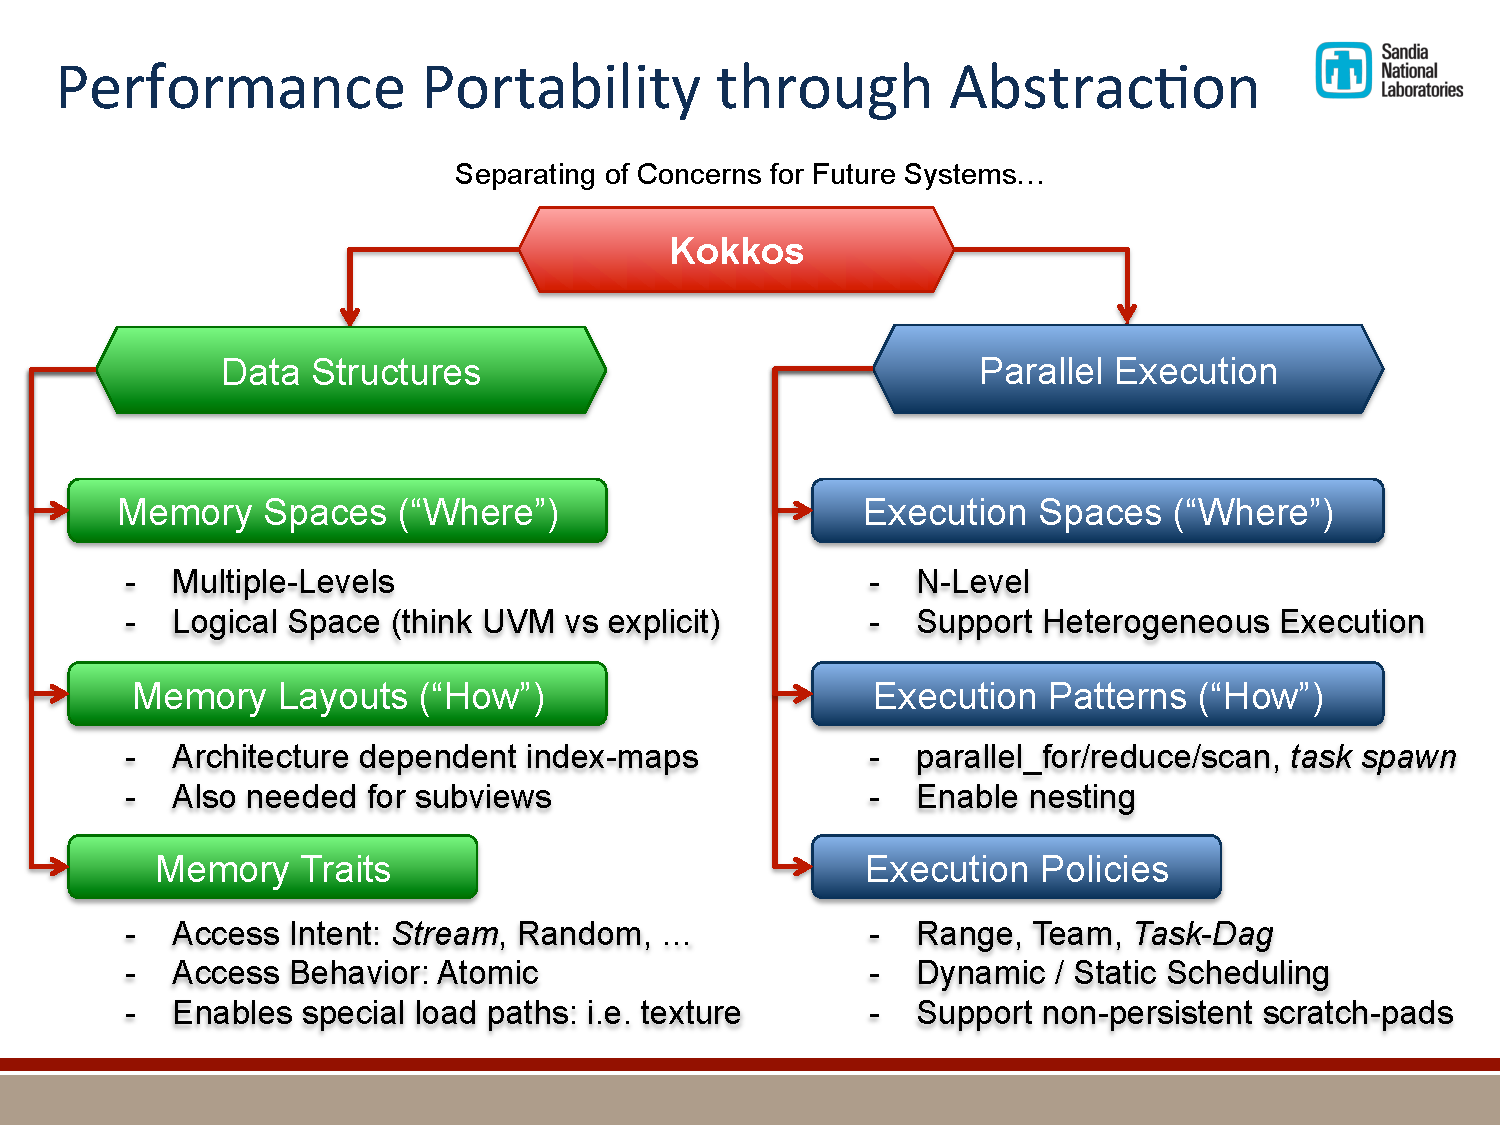
\includegraphics[width=8.0cm]{../intro/images/Kokkos-Multi-CoE_slide3}
  \end{center}

  {\small reference: \myurl{https://cfwebprod.sandia.gov/cfdocs/CompResearch/docs/Kokkos-Multi-CoE.pdf}}

\end{frame}



% remind the difference between CPU and GPU +
% the need for Kokkos
%%%%%%%%%%%%%%%%%%%%%%%%%%%%%%%%%%%%
%%%%%%%%%%%%%%%%%%%%%%%%%%%%%%%%%%%
\begin{frame}
  \frametitle{Main difference between CPU and GPU}
  
  \begin{center}
    \textbf{\textcolor{blue}{Architecture design differences between manycore GPUs and general purpose multicore CPU ?}}
    
    \only<1-4>{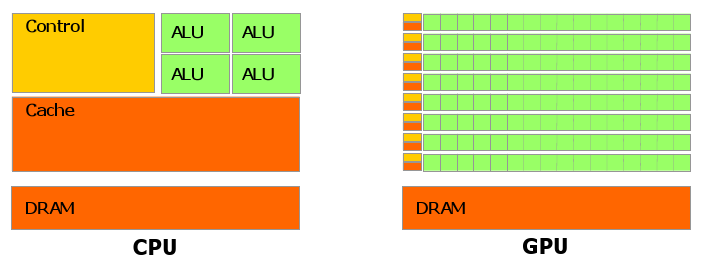
\includegraphics[height=3.5cm]{images/cpu_gpu_comparison}}

  \end{center}

\begin{itemize}

  \only<1>{
  \item \textbf{Different goals produce different designs:}
    \begin{itemize}
    \item \textcolor{red}{\textbf{CPU}}  must be good at everything, parallel or not
    \item \textcolor{blue}{\textbf{GPU}} assumes work load is highly parallel
    \end{itemize}
  }
  \only<2>{
  \item \textcolor{red}{\textbf{CPU}} design goal : optimize architecture for sequential code
    performance : \textcolor{red}{minimize latency experienced by \textbf{1 thread}}
    % latence = nb de cycle d'horloge pour acheminer des donnees de la memoire centrale jusqu'au coeur de calcul (ALU)
    % donner l'illusion d'une memoire tres rapide
    % exploiter la localite spatiale et temporelle de la memoire
    % s'il n'y avait pas de cache, les coeurs de proc serait sans arret en "stall"
    % voir l'article: http://dl.acm.org/citation.cfm?id=2692965.2682585
    % Rethinking caches for throughput processors: technical perspective
    % by Stephen W. Keckler
    
    \begin{itemize}
    \item \textcolor{red}{sophisticated} (i.e. large chip area) \textcolor{red}{control logic} for instruction-level parallelism
      (branch prediction, out-of-order instruction, etc...)
    \item \textcolor{red}{CPU have large cache memory} to reduce the instruction and
      data access latency
    \end{itemize}
  }

  \only<3>{
  \item \textcolor{blue}{\textbf{GPU}} design goal : \textcolor{blue}{maximize throughput of \textbf{all threads}}
    \begin{itemize}
    \item \# threads in flight limited by resources => lots of
      resources (registers, bandwidth, etc.)
    \item  multithreading can \textcolor{blue}{hide latency} => skip the big caches
    \item \textcolor{blue}{share control logic} across many threads
    \end{itemize}
  }

  \only<4>{
  \item \textcolor{red}{\bf CPU} : 1 thread $\Leftrightarrow$ 1 core
  \item \textcolor{blue}{\bf GPU}: nb threads $\gg$ nb cores
  }
\end{itemize}
  
\end{frame}

%%%%%%%%%%%%%%%%%%%%%%%%%%%%%%%%%%%%%%%%%%%%%%%% 
%%%%%%%%%%%%%%%%%%%%%%%%%%%%%%%%%%%%%%%%%%%%%%%% 
\begin{frame}
  \frametitle{Multidimensional array and data parallelism}

  \begin{center}
    \textcolor{violet}{\Large Memory layouts / index linearization: e.g. 2D}
  \end{center}
  
  \begin{columns}
    \begin{column}{0.5\textwidth}
      \begin{center}
        \textcolor{red}{\large row-major}
        
        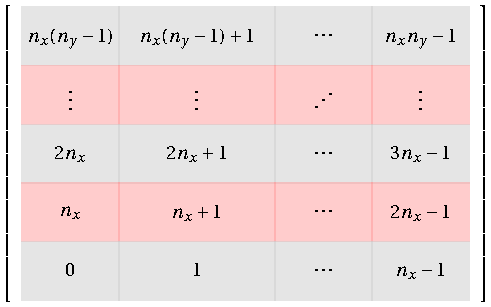
\includegraphics[width=5cm]{images/tikz/row-major}

        $\text{index} = i + n_x j$, \textcolor{red}{left layout}\\
        fast index on the left
      \end{center}
    \end{column}
    % 
    \begin{column}{0.5\textwidth}
      \begin{center}
        \textcolor{blue}{\large column-major}
        
        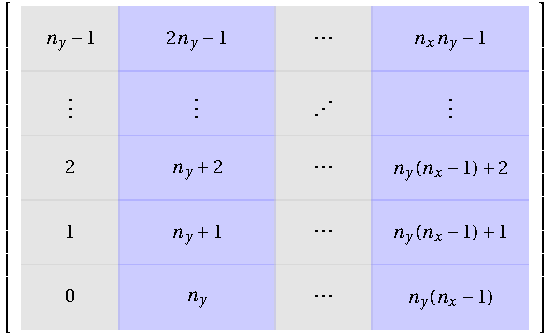
\includegraphics[width=5cm]{images/tikz/col-major}        

        $\text{index} = j + n_y i$, \textcolor{blue}{right layout}\\
        fast index on the right
      \end{center}
    \end{column}
  \end{columns}

\end{frame}

%%%%%%%%%%%%%%%%%%%%%%%%%%%%%%%%%%%%%%%%%%%%%%%% 
%%%%%%%%%%%%%%%%%%%%%%%%%%%%%%%%%%%%%%%%%%%%%%%% 
\begin{frame}[fragile=singleslide]
  \frametitle{Multidimensional array and data parallelism}

  \begin{block}{}
    {\large \textcolor{violet}{Question:}
    Assuming \textcolor{red}{left layout}, which loop would you prefer to parallelize (inner or outer) ?}    
  \end{block}
  
  \begin{columns}
    \begin{column}{0.45\textwidth}
      \begin{center}
        \textcolor{red}{\large row-major}
        
        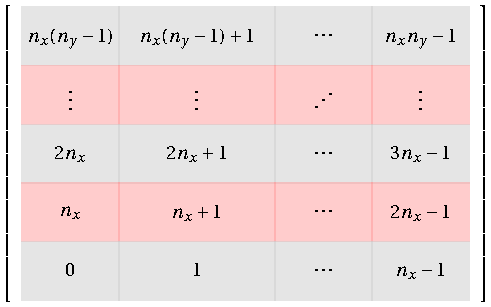
\includegraphics[width=5cm]{images/tikz/row-major}

        $\text{index} = i + n_x j$, \textcolor{red}{left layout}\\
        fast index on the left
      \end{center}
    \end{column}
    %\hspace{-1.5cm}
    \begin{column}{0.48\textwidth}
\begin{minted}{c++}
  for(int j=0; j<ny; ++j)
    for(int i=0; i<nx; ++i)
      data[i+nx*j] += 12;
\end{minted}
\begin{center}
  \textcolor{blue}{\bf Favor memory locality:}
\end{center}
\begin{itemize}
\item maximize cache usage for CPU
\item maximize memory coalescence on GPU
\end{itemize}
\begin{center}
  \textcolor{darkgreen}{\bf Different hardware $\Rightarrow$ \\ different parallelization strategies}
\end{center}
\end{column}
    \hfill
  \end{columns}
\end{frame}

%%%%%%%%%%%%%%%%%%%%%%%%%%%%%%%%%%%%%%%%%%%%%%%% 
%%%%%%%%%%%%%%%%%%%%%%%%%%%%%%%%%%%%%%%%%%%%%%%% 
\begin{frame}[fragile=singleslide]
  \frametitle{Multidimensional array and data parallelism}

  \begin{block}{}
    {\large \textcolor{violet}{Question:}
    Assuming \textcolor{red}{left layout}, which loop would you prefer to parallelize (inner or outer) ?}    
  \end{block}
  
  \begin{columns}
    \begin{column}{0.48\textwidth}
      \begin{center}
        \textcolor{red}{\large row-major}
        
        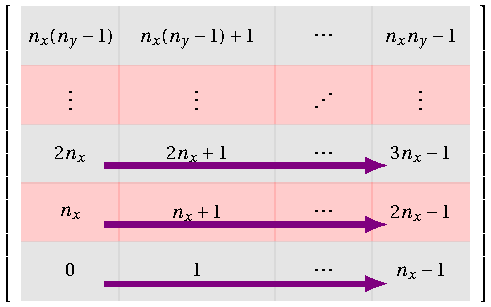
\includegraphics[width=5cm]{images/tikz/row-major-openmp}

        $\text{index} = i + n_x j$, \textcolor{red}{left layout}\\
        fast index on the left
      \end{center}
    \end{column}
    %\hspace{-1.0cm}
    \begin{column}{0.48\textwidth}
      \begin{center}
        \textcolor{violet}{\bf OpenMP // outer loop}\\
        each OpenMP thread handles {\bf 1 or more row(s)}
      \end{center}
      \begin{minted}{c++}
#pragma omp parallel
{
  #pragma omp for
  for(int j=0; j<ny; ++j)

    // vectorization loop
    // memory contiguity
    for(int i=0; i<nx; ++i)
      data[i+nx*j] += 12;
}
      \end{minted}
    \end{column}
    \hfill
  \end{columns}
\end{frame}

%%%%%%%%%%%%%%%%%%%%%%%%%%%%%%%%%%%%%%%%%%%%%%%% 
%%%%%%%%%%%%%%%%%%%%%%%%%%%%%%%%%%%%%%%%%%%%%%%% 
\begin{frame}[fragile=singleslide]
  \frametitle{Multidimensional array and data parallelism}

  \begin{block}{}
    {\large \textcolor{violet}{Question:}
    Assuming \textcolor{red}{left layout}, which loop would you prefer to parallelize (inner or outer) ?}    
  \end{block}
  
  \begin{columns}
    \begin{column}{0.48\textwidth}
      \begin{center}
        \textcolor{red}{\large row-major}
        
        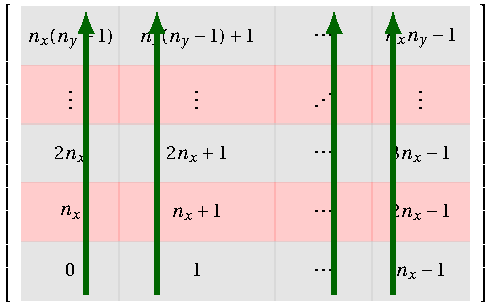
\includegraphics[width=5cm]{images/tikz/row-major-cuda}

        $\text{index} = i + n_x j$, \textcolor{red}{left layout}\\
        fast index on the left
      \end{center}
    \end{column}
    %\hspace{-1.0cm}
    \begin{column}{0.48\textwidth}
      \begin{center}
        \textcolor{darkgreen}{\bf CUDA // inner loop}\\
        each CUDA thread handles {\bf1 or more col(s)}\\
        memory coalescence
      \end{center}
      {\small
        \begin{minted}[autogobble=true]{c++}
__global__ void compute(int *data)
{
  // adjacent memory cells
  // computed by
  // neighboring threads
  int i = threadIdx.x +
      blockIdx.x*blockDim.x;
  
  for(int j=0; j<ny; ++j)
    data[i+nx*j] += 12;
}
\end{minted}
}
    \end{column}
    \hfill
  \end{columns}
\end{frame}

%%%%%%%%%%%%%%%%%%%%%%%%%%%%%%%%%%%%%%%%%%%%%%%% 
%%%%%%%%%%%%%%%%%%%%%%%%%%%%%%%%%%%%%%%%%%%%%%%% 
\begin{frame}[fragile=singleslide]
  \frametitle{Multidimensional array and data parallelism}

  \begin{block}{Conclusion}
    {\Large Don't assume \textcolor{red}{layout}, let's \textcolor{red}{chose} at compile-time !}
  \end{block}
  
  \begin{itemize}
  \item {\bf First conclusion:}\\
    if we keep the same memory layout, \textcolor{violet}{\bf OpenMP} and \textcolor{darkgreen}{\bf CUDA} \textcolor{red}{\bf disagree} on which loop should be parallelized to optimize for their respective hardware target.
  \item \textcolor{blue}{\bf How can we make portable code ?}
  \item Note that swapping memory layout and {\tt for loops} is {\bf involutive}
  %\item instead of swapping loops, swap memory layout
  \item \textcolor{orange}{\bf Kokkos answer:} make memory layout abstract (since a good memory layout is hardware dependent), fixed at compile-time\\
    access $data(i,j)$
    \begin{itemize}
    \item On \textcolor{violet}{\bf OpenMP} $data(i,j)$ actually means accessing $dataPtr[Ny*i+j]$
    \item On \textcolor{darkgreen}{\bf Cuda} $data(i,j)$ actually means accessing $dataPtr[i+Nx*j]$
    \end{itemize}
  \end{itemize}
  
\end{frame}

%%%%%%%%%%%%%%%%%%%%%%%%%%%%%%%%%%%%%%%%%%%%%%%% 
%%%%%%%%%%%%%%%%%%%%%%%%%%%%%%%%%%%%%%%%%%%%%%%% 
\begin{frame}[fragile=singleslide]
  \frametitle{Multidimensional array and data parallelism}

  \begin{block}{Conclusion}
    {\Large Don't assume \textcolor{red}{layout}, let's \textcolor{red}{chose} at compile-time !\\
    $\Rightarrow$ \textcolor{red}{\textbf{and make it hardware aware.}}}
  \end{block}
  
  \begin{columns}
    \begin{column}{0.45\textwidth}
      \begin{center}
        \textcolor{black}{\large left layout / CUDA}\\
        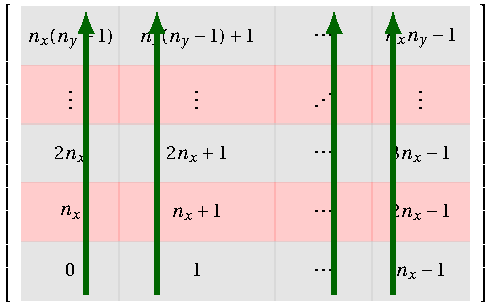
\includegraphics[width=2.8cm]{images/tikz/row-major-cuda}

        \textcolor{black}{\large right layout / OpenMP}\\
        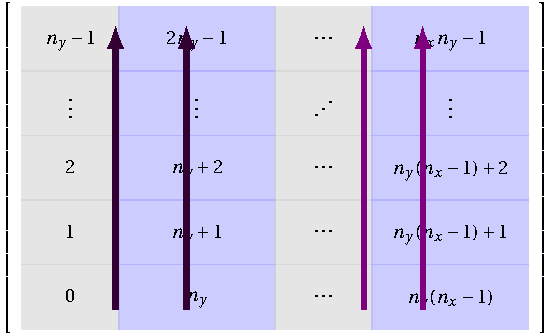
\includegraphics[width=2.8cm]{images/tikz/col-major-kokkos-openmp}

      \end{center}
    \end{column}
    %\hspace{-1.5cm}
    \begin{column}{0.45\textwidth}
      \begin{center}
        \textcolor{orange}{\bf Kokkos parallel version for both CUDA/OpenMP}
      \end{center}
      \begin{minted}{c++}
Kokkos::parallel_for(nx,
   KOKKOS_LAMBDA(int i) {
     for (int j=0; j<ny; ++j)
       data(i,j) += 12;
   }
);
      \end{minted}
    \end{column}
    \hfill
  \end{columns}
\end{frame}


%%%%%%%%%%%%%%%%%%%%%%%%%%%%%%%%%%%%%%%%%%%%%%%%
%%%%%%%%%%%%%%%%%%%%%%%%%%%%%%%%%%%%%%%%%%%%%%%%
\begin{frame}
  \frametitle{(Pre-)Exascale machines - architecture diversity !}

  \begin{itemize}
  \item \textcolor{red}{\bf \large US}: Summit , Sierra $\Rightarrow$ mostly OpenPower (IBM P9 + Nvidia V100), GPU-based architecture, \#2 and \#3 @top500; exascale machines announced
    \begin{itemize}
     \item \myhref{https://www.nextplatform.com/2019/03/18/intel-to-take-on-openpower-for-exascale-dominance-with-aurora/}{Aurora} (Argonne NL, 2022): Intel \myhref{https://www.nextplatform.com/2018/12/16/intel-unfolds-roadmaps-for-future-cpus-and-gpus/}{Xe GPU}
     \item \myhref{https://www.nextplatform.com/2019/05/07/cray-amd-tag-team-on-1-5-exaflops-frontier-supercomputer/}{Frontier} (Oak Ridge NL, 2021 ?): AMD EPYC + Radeon Instinct GPU
    \end{itemize}
  \item \textcolor{blue}{\bf \large China:}
    \begin{itemize}
    \item Phytium FT2000/64 ARM chips + Matrix2000 GPDSP accelerators $\Rightarrow$ \#6 @top500, Tianhe-2A, 61 PFlops
    \item 260-core Shenwei, \textcolor{blue}{\bf homegrow technology} hardware + software (C++/fortran compiler + OpenACC) $\Rightarrow$ \#4 @top500 , Sunway TaihuLight, 105 PFlops
    \item Dhyana, AMD-licenced x86 multicore (300 M\$), identical to AMD EPYC
      % https://www.top500.org/news/china-reveals-third-exascale-prototype/
    \end{itemize}

  \item \textcolor{violet}{\bf \large Japan:} \myhref{https://postk-web.r-ccs.riken.jp/spec.html}{\bf Fugaku}(Fujitsu, ARM, RIKEN)  A64FX ARM (\textcolor{violet}{\bf home grown}, started in 2014, \textcolor{violet}{\bf \#1 @top500 (Nov. 2020)}, 900 M\$), GPU, etc ...
    % https://www.hpcwire.com/2018/09/05/no-go-for-glofo-at-7nm-and-the-fujitsu-a64fx-post-k-cpu/
    % https://www.top500.org/news/fujitsu-reveals-details-of-processor-that-will-power-post-k-supercomputer/
    % http://www.fujitsu.com/jp/Images/20180821hotchips30.pdf
    % https://www.theregister.co.uk/2018/08/22/fujitsu_post_k_a64fx/
  \item \textcolor{darkgreen}{\bf \large Europe} : new organization EuroHPC (2018), EC H2020 budget ($\sim$ 500 M\euro{} per year)\\
    \textcolor{darkgreen}{\bf home grown} (EPI) ARM and RISC-V architecture, early stage%just starting development
    % https://www.top500.org/news/european-program-to-develop-supercomputing-chips-begins-to-take-shape/
    % mettre une EPI roadmap
    % EuroHPC (Nov. 2018 - 2026)
    % EuroHPC, Exascale not before 2022 : https://www.youtube.com/watch?v=y7_VvcIKJnI
    % EuroHPC 2 exascale machines (500 M€)
    % EuroHPC 2 pre-exascale machines in 2021 (240 M€)
  \end{itemize}

  %{\tiny \myurl{https://www.nextplatform.com/2016/07/11/chinas-triple-play-pre-exascale-systems/}}

\end{frame}

%%%%%%%%%%%%%%%%%%%%%%%%%%%%%%%%%%%
%%%%%%%%%%%%%%%%%%%%%%%%%%%%%%%%%%%
\begin{frame}
  \frametitle{Motivations for performance portability}

  \begin{itemize}
  \item {\Large What is performance portability ?}
    \begin{itemize}
    \item \textcolor{violet}{\large \bf (Re)write your code once, (try to) run {\it efficiently} everywhere}
    \item By everywhere, we mean : Multicore Intel/ARM and Nvidia/AMD GPUs
    \item \textcolor{violet}{\bf High-level approach:} as much as possible (if possible) hide hardware details to the (physicist / applied math) software developer
    \item \myhref{https://performanceportability.org}{https://performanceportability.org}
    \item \myhref{https://asc.llnl.gov/doe-coe-mtg-2016}{1st annual DOE Performance Portability Meeting (2016)}
    \end{itemize}
  \item {\large Is that \textcolor{darkgreen}{\bf possible} ?}\\ How ?\\ Which programming model ?\\ Which language ?\\ Which compiler ? $\Rightarrow$ large combinatorics
  \item for the rest of this talk, i'll focus on the \myhref{https://github.com/kokkos/kokkos}{kokkos/C++} library
  \end{itemize}

\end{frame}

%%%%%%%%%%%%%%%%%%%%%%%%%%%%%%%%%%%%%%%%%%%%%%%%
%%%%%%%%%%%%%%%%%%%%%%%%%%%%%%%%%%%%%%%%%%%%%%%%
\begin{frame}
  \frametitle{Parallel programming models landscape}

  \begin{minipage}{0.73\linewidth}
    \begin{itemize}
    \item \textcolor{red}{\textbf{Low-level native language:}} \myhref{https://www.khronos.org/opencl/}{OpenCL}, \myhref{https://developer.nvidia.com/cuda-downloads}{CUDA}, \myhref{https://rocmdocs.amd.com/en/latest/Programming_Guides/Programming-Guides.html}{HIP}
    \item \textcolor{orange}{\textbf{Directive approach (code annotations)}} for multicore/GPU, ...:
      \begin{itemize}
      \item \myhref{http://www.openmp.org/}{OpenMP} 5.1 (Clang, PGI, GNU, ...), \myhref{https://pm.bsc.es/ompss-2}{OmpSs-2}
      \item \myhref{http://www.openacc.org/}{OpenACC} 2.7 (PGI, GNU, ...) \textcolor{blue}{$\Rightarrow$ Fortran codes.}
      \end{itemize}
    \item \textcolor{darkgreen}{\textbf{Other high-level library-based approaches}}:
      {
        \scriptsize
        \begin{itemize}
        \item \framebox{\myhref{https://github.com/kokkos/kokkos}{Kokkos}}, \myhref{https://github.com/LLNL/RAJA}{RAJA}, \myhref{https://github.com/alpaka-group/alpaka}{Alpaka}, \myhref{https://github.com/STEllAR-GROUP/hpx}{HPX}, \myhref{https://github.com/GridTools/gridtools}{GridTools}, \myhref{https://arrayfire.com/}{ArrayFire}...
        \item \myhref{https://www.khronos.org/sycl}{SYCL} (Khronos Group \textit{standard}), C++ high-level layer on top of OpenCL. %\textcolor{red}{\bf Still $\sim$experimental}\\
          \myhref{https://software.intel.com/content/www/us/en/develop/tools/oneapi.html}{Intel OneAPI/DPCPP} (Intel CPU/GPU/FPGA, Nvidia GPUs),\\
          \myhref{https://www.codeplay.com/products/computesuite/computecpp}{CodePlay},
          \myhref{https://github.com/illuhad/hipSYCL}{AMD and Nvidia GPUs},
          \myhref{https://github.com/keryell/triSYCL}{Keryell/Xilinx}
        \item {\bf C++-17 built-in parallelism for multicore and GPUs}, e.g.:
          \begin{itemize}
          \item Nvidia's \myhref{https://developer.nvidia.com/hpc-sdk}{hpc-sdk} (May 2020)
          \item \myhref{https://github.com/oneapi-src/oneTBB}{Intel OneAPI/TBB}
          \end{itemize}
        \end{itemize}
      }
    \end{itemize}
  \end{minipage}
  %
  \begin{minipage}{0.26\linewidth}
    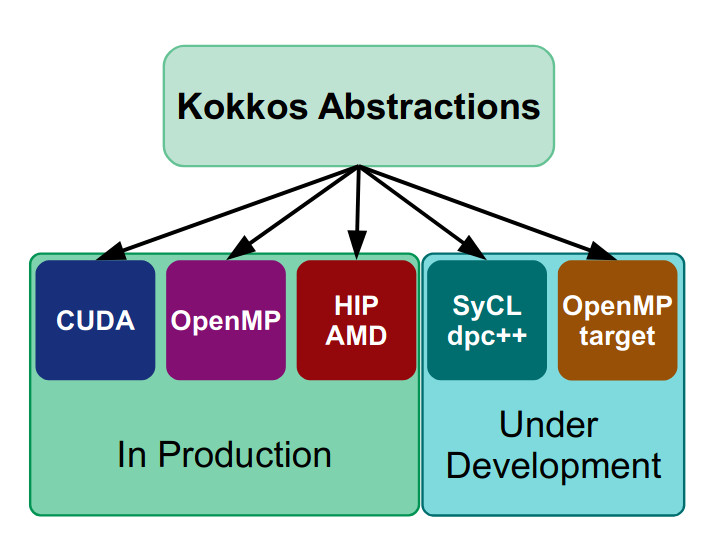
\includegraphics[width=1.3\linewidth]{./images/exascale/kokkos_backends}

    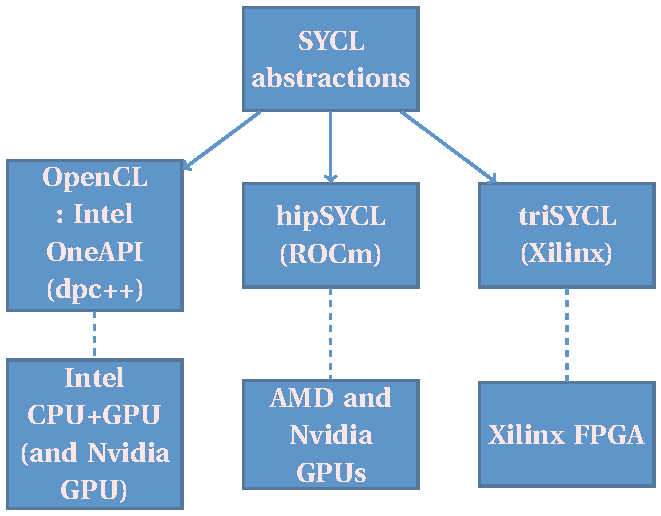
\includegraphics[width=1.3\linewidth]{./tikz/sycl}

    %\textcolor{blue}{\bf \scriptsize All these programming solutions are interconnected and inter-dependent !}

    %\begin{framed}
       {
          \scriptsize
          {\bf additionnal features:}\\
          \textcolor{violet}{\bf memory management,}\\
          \textcolor{violet}{\bf data containers}, ...
       }
    %\end{framed}

  \end{minipage}

\end{frame}

%%%%%%%%%%%%%%%%%%%%%%%%%%%%%%%%%%%%%%%%%%%%%%%%%%%%%%%%%%%%%%%%%%%
%%%%%%%%%%%%%%%%%%%%%%%%%%%%%%%%%%%%%%%%%%%%%%%%%%%%%%%%%%%%%%%%%%%
%%%%%%%%%%%%%%%%%%%%%%%%%%%%%%%%%%%%%%%%%%%%%%%%%%%%%%%%%%%%%%%%%%%
\begin{frame}
  \frametitle{Kokkos: a programming model for perf. portability}

  \only<1>{
    \begin{itemize}
    \item \textcolor{blue}{\textbf{Kokkos}} is a \textbf{C++ library} for \textcolor{violet}{\textbf{node-level parallelism}} (i.e. \textcolor{violet}{\bf shared memory}) providing abstractions for {\bf harware-aware}:

      \begin{itemize}
      \item \textcolor{red}{\textbf{parallel algorithmic patterns}}
      \item \textcolor{red}{\textbf{data containers}}
      \end{itemize}
    \item \myurl{https://kokkos.org/}
    \item Implementation relies heavily on \textbf{C++ meta-programing} to derive native low-level code (OpenMP, CUDA, HIP, SYCL...) and adapt data structure memory layout at compile-time
    \item Developped at \textcolor{violet}{\textbf{Sandia NL}} (core, CUDA, OpenMP), \textcolor{violet}{\textbf{ORNL}} (HIP, SYCL), ...
    \end{itemize}

    \textcolor{darkgreen}{\bf Goal:} {\bf write one implementation which:}
    \begin{itemize}
    \item compiles and \textcolor{blue}{\bf run on multiple archs},
    \item obtains \textcolor{blue}{\bf performant memory access pattern} across archs,
    \item can leverage \textcolor{blue}{\bf arch-specific features} where possible.
    \end{itemize}

  }
  \only<2>{
    \begin{itemize}
    \item \textcolor{darkgreen}{\textbf{Open source}}, \myurl{https://github.com/kokkos/kokkos}, since $\sim 2012$
    \item Primarily developped as a base building layer for \textbf{generic high-performance parallel linear algebra} in \myhref{https://github.com/trilinos/Trilinos}{Trilinos}
    \item Used in, e.g.:
      \begin{itemize}
      \item \myhref{http://lammps.sandia.gov/}{LAMMPS} (molecular dynamics code),
        %\myhref{https://github.com/ECP-copa/ExaMiniMD}{ExaMiniMD}
      \item \myhref{https://github.com/NaluCFD/Nalu}{NALU CFD} (low-Mach wind flow),
      \item \myhref{https://sparta.sandia.gov/}{SPARTA/DSMC} (rarefied gas flow), \myhref{}{SPARC} (CFD, RANS, LES, hypersonic flow)
      \item \myhref{https://github.com/SNLComputation/Albany}{Albany} (fluid/solid,...)
      \item \myhref{http://uintah.utah.edu/}{Uintah} (structured AMR, combustion, radiation)
        % \item list of codes using Kokkos: \myurl{https://github.com/kokkos/kokkos/issues/1950}
      %\item \myhref{https://github.com/kokkos/kokkos/issues/1950}{list of codes using Kokkos}
      \end{itemize}

      % \item Goal: \textcolor{orange}{\textbf{ISO/C++ 2020 Standard}} subsumes Kokkos abstractions~\footnote{\scriptsize see mdspan proposal \myurl{https://github.com/kokkos/array_ref}}
    \end{itemize}
  }

  \only<2>{
  \begin{columns}
    \begin{column}{0.34\linewidth}
      Strong involvement in \textcolor{orange}{\textbf{ISO/C++ 2020 Standard}}\\
      Make Kokkos a sliding window of future c++ features
    \end{column}
    \begin{column}{0.65\linewidth}
      \begin{center}
        \includegraphics<1-2>[width=5cm]{images/perf_portability/kokkos_summary}
      \end{center}
    \end{column}
  \end{columns}
  \vfill
  {
    \scriptsize see mdspan proposal \myurl{https://github.com/kokkos/mdspan}\\
    \myurl{https://arxiv.org/abs/2010.06474}
  }
}

\end{frame}

%%%%%%%%%%%%%%%%%%%%%%%%%%%%%%%%%%%%%%%%%%%%%%%%%%%%%%%%%%%%%%%%%%%
%%%%%%%%%%%%%%%%%%%%%%%%%%%%%%%%%%%%%%%%%%%%%%%%%%%%%%%%%%%%%%%%%%%
%%%%%%%%%%%%%%%%%%%%%%%%%%%%%%%%%%%%%%%%%%%%%%%%%%%%%%%%%%%%%%%%%%%
\begin{frame}
  \frametitle{Kokkos: a programming model for perf. portability}

  \begin{center}
    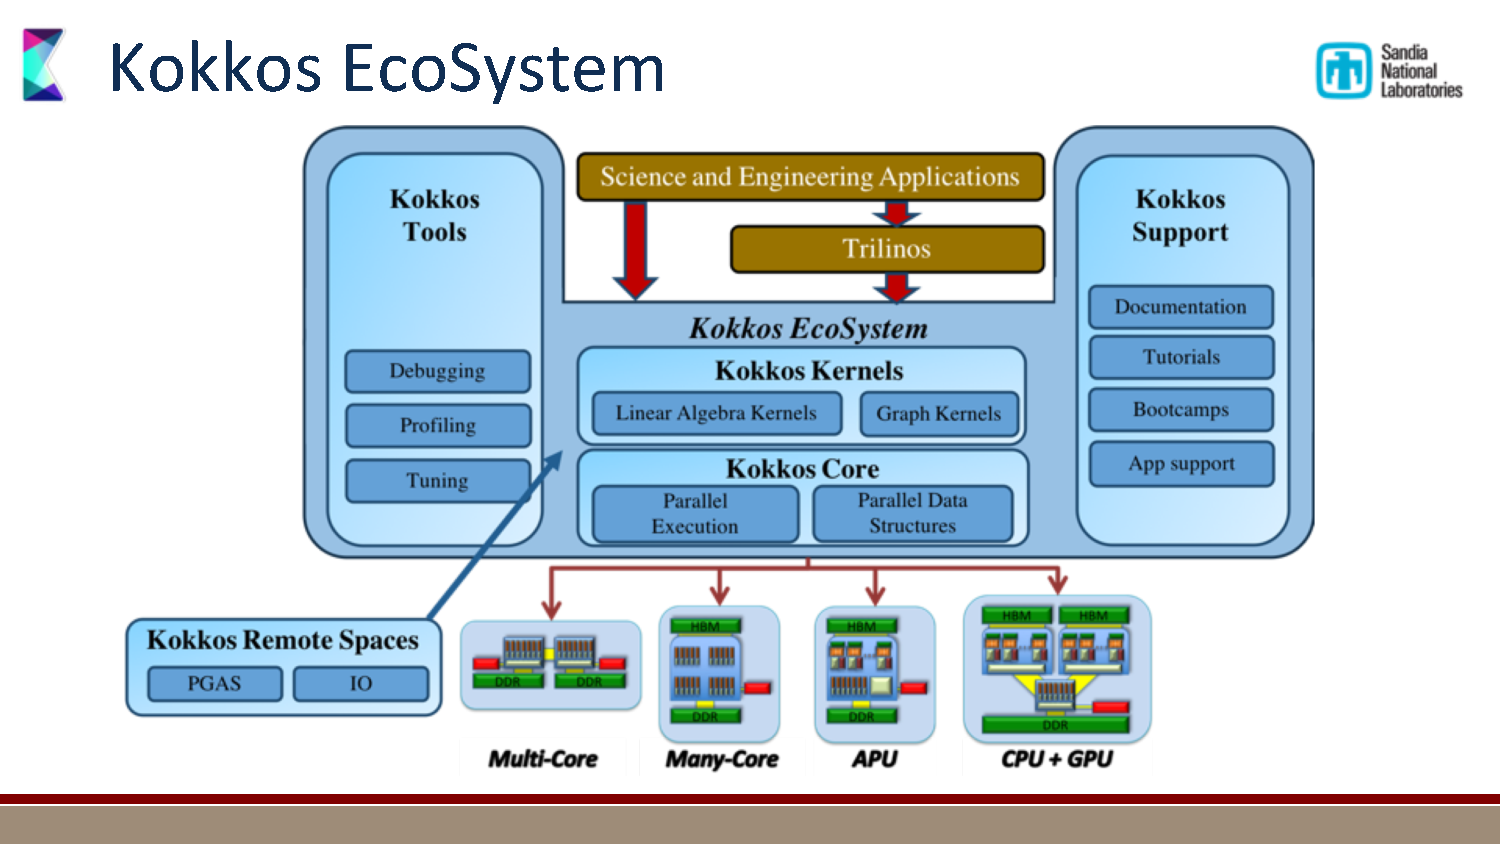
\includegraphics[width=0.8\linewidth]{images/kokkos/trott1}
  \end{center}

  { \tiny
    \begin{itemize}
    \item \myhref{https://github.com/kokkos/kokkos-kernels}{Kokkos-kernels} (many dense/sparse BLAS problems, ...), \myhref{https://github.com/kokkos/simd-math}{simd-math}, \myhref{https://github.com/ECP-copa/Cabana}{Cabana} (for particle-based codes)
    \item \myhref{https://github.com/kokkos/kokkos-fortran-interop}{Fortran compatibility layer} (REX code \myhref{https://ecpannualmeeting.com/assets/overview/sessions/XGC_ECP_2020.pptx}{XGC-Cabana}, Plasma physics, Gyrocinetics, particle-in-cell)
    \item \myhref{https://github.com/kokkos/pykokkos-base}{pykokkos-base} (\myhref{https://github.com/pybind/pybind11}{pybind11}-based API mapping + memory, numpy/cupy interoperability), \myhref{https://github.com/kokkos/pykokkos}{pykokkos} (decorator + python to C++ translation)
    \item \myhref{https://prod-ng.sandia.gov/techlib-noauth/access-control.cgi/2017/1710464.pdf}{Task-DAG parallelism (CPU / GPU)}
    \end{itemize}
  }

  source: C. Trott, DOE Performance Portability Meeting, April 2019
\end{frame}

%%%%%%%%%%%%%%%%%%%%%%%%%%%%%%%%%%%
%%%%%%%%%%%%%%%%%%%%%%%%%%%%%%%%%%%
% \begin{frame}
%   \frametitle{C++ Kokkos library summary}

%   \begin{itemize}
%   %\item See GTC2017 session \textcolor{violet}{S7344 - Kokkos ? The C++ Performance Portability Programming Model} (C. Trott and H.C. Edwards).
%   \item Framework for efficient \textcolor{RedOrange}{\bf node-level parallelism (CPU, GPU, ...)}
%   \item Provides
%     \begin{itemize}
%     \item \textcolor{blue}{\bf Computationnal parallel patterns} (for, reduce, scan, ...)
%     \item \textcolor{violet}{\bf Hardware aware memory containers}: e.g. {\bf A multi-dimensionnal data container with hardware adapted memory layout}
%     \item Support for multiple backends:
%       {\scriptsize
%         \begin{itemize}
%         \item OpenMP (x86, ARM, IBM, ...)
%         \item pthreads
%         \item OpenMP target (GPU, ...),
%         \item CUDA (Nvidia GPU, ...),
%         \item HIP (AMD and Nvidia GPU),
%         \item SYCL (Intel CPU and GPU, Nvidia, ...)
%         \item HPX
%         \end{itemize}
%       }
%     \item Additionnal sub-projects: \myhref{https://github.com/kokkos/kokkos-kernels}{kokkos-kernels} (BLAS, sparse BLAS, Graph), \myhref{https://github.com/kokkos/simd-math}{Kokkos::simd}, \myhref{https://github.com/kokkos/kokkos-python}{python bindings}, ...

%     \end{itemize}
%   % \item Provides some {\bf \textcolor{RedOrange}{high-level (abstract) concepts}} as template C++ classes:
%   %   \begin{itemize}
%   %   \item A \textcolor{red}{\bf kokkos device:} \texttt{Kokkos::Cuda, Kokkos::OpenMP, Kokkos::Pthreads, Kokkos::Serial},...
%   %   \item concepts controlled by C++ template meta-programing: \textcolor{darkgreen}{\bf execution space, memory space, memory layout, ...}
%   %   \item \textcolor{blue}{\bf Computationnal parallel patterns} (for, reduce, scan, ...) controlled with a {\bf execution policy} (i.e. how many iterations, teams, ...)
%   %   \end{itemize}
%   % \item \textcolor{violet}{\bf \texttt{Kokkos::View}}: {\bf A multi-dimensionnal data container with hardware adapted memory layout} \\
%   %   % with ability to mirror view between memory spaces, ...
%   %   {\small
%   %     -\;\textcolor{violet}{\texttt{Kokkos::View<double **> data("data",NX,NY);}} // 2D array with sizes known at runtime\\
%   %     -\;\framebox{{\bf How do I access data ?} \texttt{data(i,j)} !}
%   %   }
%   \item Mostly a header library (C++ metaprogramming)
%   %\item build system / module load / etc ... (?)
%   \end{itemize}

% \end{frame}

%%%%%%%%%%%%%%%%%%%%%%%%%%%%%%%%%%%
%%%%%%%%%%%%%%%%%%%%%%%%%%%%%%%%%%%
% \begin{frame}
%   \frametitle{C++ Kokkos library summary}

%   % I started using Kokkos in June 2016, shortly developped 2D Hydro MUSCL-Hancok 2nd order scheme.

%   \begin{itemize}
%   \item {\bf What does it mean hardware aware memory containers ?}
%   \item Most commonly in a C/C++, {\bf multi-dimensionnal array access} is done through {\bf \textcolor{red}{index linearization}} (row or column-major in 2D):
%     $$ \mathbf{index} = \mathbf{i} + nx * \mathbf{j}  + nx*ny * \mathbf{k}$$
%   \item {\bf Fortran} (column-major format) vs {\bf C/C++} (row-major format)
%   \item There is no reason to favour one layout versus the other
%     \begin{itemize}
%     \item column-major is better for vectorization on CPU architecture
%     \item row-major is better for high througput architecture e.g. GPU (memory coalescence)
%     \item $\Rightarrow$ \textcolor{orange}{\bf Kokkos allows to chose memory layout at compile time}
%     \end{itemize}
%   \item In Kokkos, one should/must avoid this index linearization at the user level, let \texttt{Kokkos::View} do this job (\textcolor{darkgreen}{\bf decided at compile-time, hardware adapted})
%     $$ \text{data}(i,j,k) $$
%     % \begin{itemize}
%     % \item 1D \texttt{Kokkos::View} with user-defined index linearization + 1D Iteration range
%     % \item \textcolor{blue}{2D \texttt{Kokkos::View}  + 1D flat Iteration range} {\bf (used in this work)}
%     % \item 2D \texttt{Kokkos::View}  + 2D (\texttt{Kokkos::MDRange} Kernel policy) : still an experimental feature
%     % \end{itemize}
%   %\item \texttt{Kokkos::MDRange} is functional, but was generating kernels with some performance loss, will surely be solved shortly by Kokkos core developpers.
%   %\item See also new developpement on hierarchical task-data parallelism, session S7253 (Monday 8th, room 211B).
%   \end{itemize}

%   % Some personnal views / experience as an external Kokkos user

% \note[item]{Let me brievely add a comment on memory layout, which is an important feature. With kokkos, array linearization is a low-level implementation detail, that must be abstracted away, if I may say. This way, the end-programmer only access data using a multi-index set, linearization is done in an hardware-aware way by kokkos at compile time, once the target device has been specified.}

% \end{frame}

%%%%%%%%%%%%%%%%%%%%%%%%%%%%%%%%%%%%%%%%%%%%%%%%%%%%%%%%%%%%%%%%%%%%%%%%
%%%%%%%%%%%%%%%%%%%%%%%%%%%%%%%%%%%%%%%%%%%%%%%%%%%%%%%%%%%%%%%%%%%%%%%%
\begin{frame}
  \frametitle{Kokkos - Documentation}

  \begin{itemize}
  %\item PDF documentation in kokkos source tree : \texttt{doc/Kokkos\_PG.pdf} (programming guide)
  %\item \myhref{http://www.stack.nl/~dimitri/doxygen/}{Doxygen} can only be built from inside \myhref{https://github.com/trilinos/Trilinos}{Trilinos source tree}\\
   % Version of the day can be browsed at \myurl{https://trilinos.org/docs/dev/packages/kokkos/doc/html/index.html}
  \item \myhref{https://github.com/kokkos/kokkos-tutorials/wiki/Kokkos-Lecture-Series}{Kokkos video lectures + slides} : \myurl{https://github.com/kokkos/kokkos-tutorials/wiki/Kokkos-Lecture-Series}
  \item \myhref{https://github.com/kokkos/kokkos-tutorials}{Kokkos tutorial} : \myurl{https://github.com/kokkos/kokkos-tutorials}
  \item Kokkos source code itself, reading unit tests code is also very helpful
  \end{itemize}

\end{frame}


%%%%%%%%%%%%%%%%%%%%%%%%%%%%%%%%%%%%%%%%%%%%%%%%%%%%%%%%%%%%%%%%%%% 
%%%%%%%%%%%%%%%%%%%%%%%%%%%%%%%%%%%%%%%%%%%%%%%%%%%%%%%%%%%%%%%%%%% 
%%%%%%%%%%%%%%%%%%%%%%%%%%%%%%%%%%%%%%%%%%%%%%%%%%%%%%%%%%%%%%%%%%% 
\begin{frame}
  \frametitle{Kokkos Concepts (1) - the abstract machine model}

  \begin{itemize}
  \item Kokkos defines an abstract machine model for future large shared-memory nodes made of 
    \begin{itemize}
    \item \textcolor{blue}{\textbf{latency-oriented cores}} (contemporary CPU core)
    \item \textcolor{orange}{\textbf{throughput-oriented cores}} (GPU, ...)
    \end{itemize}
  \end{itemize}

  \begin{center}
    \begin{figure}
      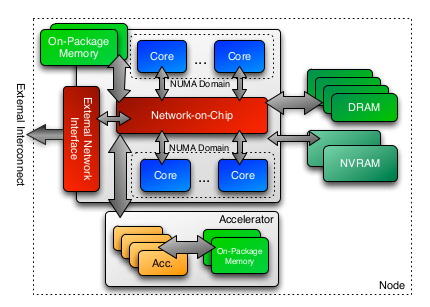
\includegraphics[width=5cm]{images/kokkos_machine_model}
      \caption{Conceptual model of a future HPC node. (Kokkos User's Guide).}
      \end{figure}
  \end{center}

\end{frame}


%%%%%%%%%%%%%%%%%%%%%%%%%%%%%%%%%%%%%%%%%%%%%%%%%%%%%%%%%%%%%%%%%%% 
%%%%%%%%%%%%%%%%%%%%%%%%%%%%%%%%%%%%%%%%%%%%%%%%%%%%%%%%%%%%%%%%%%% 
%%%%%%%%%%%%%%%%%%%%%%%%%%%%%%%%%%%%%%%%%%%%%%%%%%%%%%%%%%%%%%%%%%% 
\begin{frame}[fragile=singleslide]
  \frametitle{Kokkos Concepts (2) - What is a device ?}

  \begin{itemize}
  \item A \textcolor{red}{\textbf{Kokkos device}}: 
  \item From a C++ API design point of view, Kokkos defines several c++ class for a \textcolor{red}{device} in \texttt{core/src}, e.g.
    \begin{itemize}
    \item Kokkos::Cuda, Kokkos::OpenMP, Kokkos::Pthreads, Kokkos::Serial
    \item \textcolor{blue}{\textit{device} = execution space + memory space}
    \end{itemize}
  \item Each \textit{Kokkos device} pre-defines some types
  \item Example \textcolor{red}{\textbf{Kokkos device}} (not required for a user, only Kokkos developper), e.g.\\
    {\tiny
      \begin{minted}{c++}
        class Cuda {
          public:
          // Tag this class as a kokkos execution space
          typedef Cuda                  execution_space ;
          
          #if defined( KOKKOS_USE_CUDA_UVM )
          // This execution space's preferred memory space.
          typedef CudaUVMSpace          memory_space ;
          #else
          // This execution space's preferred memory space.
          typedef CudaSpace             memory_space ;
          #endif
          
          // This execution space preferred device_type
          typedef Kokkos::Device<execution_space,memory_space> device_type;
          
          // The size_type best suited for this execution space.
          typedef memory_space::size_type  size_type ;
          
          // This execution space's preferred array layout.
          typedef LayoutLeft            array_layout ;
          ...
        } // end class Cuda
        \end{minted}
      }
  \end{itemize}

\end{frame}

%%%%%%%%%%%%%%%%%%%%%%%%%%%%%%%%%%%%%%%%%%%%%%%%%%%%%%%%%%%%%%%%%%% 
%%%%%%%%%%%%%%%%%%%%%%%%%%%%%%%%%%%%%%%%%%%%%%%%%%%%%%%%%%%%%%%%%%% 
%%%%%%%%%%%%%%%%%%%%%%%%%%%%%%%%%%%%%%%%%%%%%%%%%%%%%%%%%%%%%%%%%%% 
\begin{frame}
  \frametitle{Kokkos Concepts (3) - execution space, memory space}

  \begin{itemize}
  \item \textcolor{blue}{\textbf{Execution space:}} Where should a parallel contruct (\texttt{parallel\_for}, \texttt{parallel\_reduce}, ...) be executed\\
    \begin{itemize}
    \item Special case: \texttt{class HostSpace}, special device (always defined) where execution space is either (Serial, Pthread or OpenMP).
    \item Each execution space is equipped with a \texttt{fence}: \texttt{Kokkos::Cuda::fence()}
    \end{itemize}
  \item \textcolor{blue}{\textbf{Memory space:}} Where / how data are allocated in memory (HostSpace, CudaSpace, CudaUVMSpace, CudaHostPinnedSpace, HBWSpace, ...)
  \item \textcolor{blue}{\textbf{Memory layout}} (come back later on that)
  \item Other concepts:
    \begin{itemize}
    \item Execution policy: used to modify a parallel thread dispatch
    \end{itemize}
  \item \textcolor{red}{Multiple execution / memory space} can be used in a single application\\
    See for example in Kokkos sources \texttt{example/tutorial/Advanced\_View/07\_Overlapping\_DeepCopy}\\
    Though, take care that currently, Cuda stream are completely mapped into Kokkos API~\footnote{Will be implemented in the coming months}; meanwhile Cuda streams can be used directly (but looses portability); 
  \end{itemize}

\end{frame}



\subsection{Build Kokkos}
%%%%%%%%%%%%%%%%%%%%%%%%%%%%%%%%%%%%%%%%%%%%%%%%%%%%%%%%%%%%%%%%%%%%%%%% 
%%%%%%%%%%%%%%%%%%%%%%%%%%%%%%%%%%%%%%%%%%%%%%%%%%%%%%%%%%%%%%%%%%%%%%%% 
\begin{frame}
  \frametitle{Hands-On 0: Build kokkos (1)}
  
  \textbf{0. Kokkos is still experimental, but moving fast: use git sources}
  
  \textbf{1. Get Kokkos sources, development branch - don't try to build yet !}
  \begin{itemize}
  \item \textcolor{blue}{Practicals on \texttt{ouessant}:}\\
    \textcolor{darkgreen}{\texttt{1. mkdir \$HOME/kokkos-tutorial; cd \$HOME/kokkos-tutorial}}\\
    some kokkos tutorial examples have a Makefile configured for using that precise location.\\
    \textcolor{darkgreen}{\texttt{2. git clone https://github.com/kokkos/kokkos}}\\
    \textcolor{darkgreen}{\texttt{3. cd kokkos; git checkout develop}}
  \end{itemize}
  
\end{frame}

%%%%%%%%%%%%%%%%%%%%%%%%%%%%%%%%%%%%%%%%%%%%%%%%%%%%%%%%%%%%%%%%%%%%%%%% 
%%%%%%%%%%%%%%%%%%%%%%%%%%%%%%%%%%%%%%%%%%%%%%%%%%%%%%%%%%%%%%%%%%%%%%%% 
\begin{frame}
  \frametitle{Hands-On 0: Build kokkos (2)}

  \textbf{2. How to build and use}
  \begin{enumerate}
  \item \textcolor{red}{\textbf{As a regular library (standalone Makefile, installed library):}} \\
    \begin{itemize}
    \item {\bf not recommended} for production level (see below), {\bf OK for testing and building examples}
    \item use \texttt{generate\_makefile.bash}, then \texttt{make kokkoslib; make install}\\
      Then use a \textit{modulefile} to configure the environment\\
      Kokkos examples (inside source) can be built that way, as well as \myhref{https://github.com/kokkos/kokkos-tutorials}{Kokkos-tutorials}
    \end{itemize}
  \item \textcolor{blue}{\textbf{Embedded Kokkos source files in your application}}
    \begin{itemize}
    \item Why ?
    \item $\Rightarrow$ Kokkos by design has {\bf many different configurations possible} (hardware adaptability, heavily relies on C++ metaprograming - compile timing )
    \item $\Rightarrow$ best practice advice : better compile kokkos as part as the target application (same flags, same compiler, etc...)
    \item $\Rightarrow$ \textcolor{blue}{\bf recommended use}:
    \textcolor{darkgreen}{\bf standalone \myhref{https://cmake.org/}{cmake} + kokkos sources embedded in your application} (we'll see a skeleton app)
    \end{itemize}
  \item There exists another cmake-based build sytem, but relies on a third-party tools \myhref{https://tribits.org/}{TriBITS}. Right now this can only be used used when Kokkos is build inside \myhref{https://github.com/trilinos/Trilinos}{Trilinos} (heterogeneous distributed sparse and dense linear algebra package).
  \end{enumerate}
 
\end{frame}

%%%%%%%%%%%%%%%%%%%%%%%%%%%%%%%%%%%%%%%%%%%%%%%%%%%%%%%%%%%%%%%%%%%%%%%% 
%%%%%%%%%%%%%%%%%%%%%%%%%%%%%%%%%%%%%%%%%%%%%%%%%%%%%%%%%%%%%%%%%%%%%%%% 
\begin{frame}
  \frametitle{Hands-On 0: Build kokkos (3)}

  {\bf \textcolor{red}{About standalone Makefile} and environment variables settings for building on multiple architectures}

  \begin{itemize}
  \item The following variables are usefull when building some of the tutorial examples :
    \begin{itemize}
    \item \texttt{KOKKOS\_PATH}: path to Kokkos source dir
    \item \texttt{KOKKOS\_DEVICES}: define possible execution spaces: CUDA, OpenMP, Pthreads, Serial, ...
    \item \texttt{KOKKOS\_ARCH}: used to customize compiler flags; e.g. Power8, Kepler35, SNB, KNL, ARMv80, ROCm, ...
    \end{itemize}
  \item When building for \textcolor{darkgreen}{\bf CUDA device}, you'll need to use Kokkos' own compiler wrapper: \textcolor{darkgreen}{\texttt{\bf nvcc\_wrapper}} (included in Kokkos sources), not just \texttt{nvcc}
  \item \textcolor{red}{When building Kokkos and aiming at an installed Kokkos}, the same information (in a different form) is passed to script \texttt{generate\_makefile.bash}\\
    Just type \texttt{./generate\_makefile.bash \--\--help} at top-level Kokkos sources
  \item \textcolor{blue}{When using Kokkos embedded in your application}, these variables must be set on the \texttt{make} command line.
  \end{itemize}
  
\end{frame}
  
%%%%%%%%%%%%%%%%%%%%%%%%%%%%%%%%%%%%%%%%%%%%%%%%%%%%%%%%%%%%%%%%%%%%%%%% 
%%%%%%%%%%%%%%%%%%%%%%%%%%%%%%%%%%%%%%%%%%%%%%%%%%%%%%%%%%%%%%%%%%%%%%%% 
\begin{frame}
  \frametitle{Hands-On 0: Build kokkos (4)}

  \begin{itemize}
  \item \textcolor{blue}{\textbf{Example build configurations (for an installed Kokkos)}}
    \begin{itemize}
    \item For \texttt{ouessant}, see file \texttt{doc/readme\_build\_kokkos\_ouessant} in the provided archive
    \item Serial (mostly for testing)\\
      \texttt{../generate\_makefile.bash --with-serial --prefix=\$HOME/local/kokkos\_serial}
    \item \textbf{OpenMP}\\
      \texttt{../generate\_makefile.bash --with-openmp --prefix=\$HOME/local/kokkos\_openmp\_dev}
    \item \textbf{CUDA (+ OpenMP)}; typical configuration\\
      \texttt{../generate\_makefile.bash --with-cuda --arch=Pascal60 --prefix=\$HOME/local/kokkos\_cuda\_lambda\_openmp --with-cuda-options=enable\_lambda --with-openmp --with-hwloc=/usr}
    \end{itemize}
  \item \textcolor{darkgreen}{\textbf{After installation}} (\texttt{make kokkoslib; make install;}) the file \textbf{\texttt{Makefile.kokkos}} is created, and designed to be reused in your application build system.
  \item \textbf{Two choices for integrating Kokkos in your app:}
    \begin{itemize}
    \item Use an existing Makefile from Kokkos tutorial, examples, ...
    \item Use your own build system ({\bf cmake recommended}): there can be a quite large combinatorics of \texttt{DEVICES}, \texttt{ARCH}, compilers, compiler options, ...
    \end{itemize}
  \end{itemize}
  
\end{frame}

%%%%%%%%%%%%%%%%%%%%%%%%%%%%%%%%%%%%%%%%%%%%%%%%%%%%%%%%%%%%%%%%%%%%%%%% 
%%%%%%%%%%%%%%%%%%%%%%%%%%%%%%%%%%%%%%%%%%%%%%%%%%%%%%%%%%%%%%%%%%%%%%%% 
\begin{frame}
  \frametitle{Kokkos - Documentation}

  \begin{itemize}
  \item PDF documentation in kokkos source tree : \texttt{doc/Kokkos\_PG.pdf} (programming guide)
  \item \myhref{http://www.stack.nl/~dimitri/doxygen/}{Doxygen} can only be built from inside \myhref{https://github.com/trilinos/Trilinos}{Trilinos source tree}\\
    Version of the day can be browsed at \myurl{https://trilinos.org/docs/dev/packages/kokkos/doc/html/index.html}
  \item Kokkos source code itself, reading unit tests code is also helpful
  \end{itemize}

  Additionnal resources:

  \begin{itemize}
  \item Tutorial slides and codes: \\
    \myurl{https://github.com/kokkos/kokkos-tutorials}
  \end{itemize}
  
\end{frame}

%%%%%%%%%%%%%%%%%%%%%%%%%%%%%%%%%%%%%%%%%%%%%%%%%%%%%%%%%%%%%%%%%%%%%%%% 
%%%%%%%%%%%%%%%%%%%%%%%%%%%%%%%%%%%%%%%%%%%%%%%%%%%%%%%%%%%%%%%%%%%%%%%% 
\begin{frame}[fragile=singleslide]
  \frametitle{Kokkos - initialize / finalize}

  \begin{itemize}
  \item \texttt{Kokkos::initialize / finalize}
    %// introspection on configuration options
    {\small\begin{minted}{c++}
        #include <Kokkos_Macros.hpp>
        #include <Kokkos_Core.hpp>
        
        int main(int argc, char* argv[]) {
          // default: initialize the host exec space
          // What exactly gets initialized depends on how kokkos
          // was built, i.e. which options was passed to
          // generate_makefile.bash
          Kokkos::initialize();
          ...
          Kokkos::finalize();
        }
      \end{minted}
    }
    %
  \item \textcolor{red}{\textbf{What's happening inside \texttt{Kokkos::initialize}}}
    \begin{itemize}
    \item Defines \textcolor{blue}{\texttt{Default Device / DefaultExecutionSpace Default memory space}} (as specified when kokkos itself was built, by order of {\bf priority}: Cuda > OpenMP > Pthreads > Serial)\\
      e.g. if \texttt{\--\--with-cuda} was not pass to \texttt{generate\_makefile.bash}, but \texttt{\--\--with-openmp} was, then \texttt{DefaultExecutionSpace} is OpenMP
    \item You can activate several execution spaces (recommended)
    %\item Defines a \textcolor{blue}{default memory space}
    \item all this information provided at compile time will internally be used inside Kokkos sources as default (hidden) template parameters
    \end{itemize}
    % 
  \end{itemize}
  %
\end{frame}

%%%%%%%%%%%%%%%%%%%%%%%%%%%%%%%%%%%%%%%%%%%%%%%%%%%%%%%%%%%%%%%%%%%%%%%% 
%%%%%%%%%%%%%%%%%%%%%%%%%%%%%%%%%%%%%%%%%%%%%%%%%%%%%%%%%%%%%%%%%%%%%%%% 
\begin{frame}[fragile=singleslide]
  \frametitle{Kokkos - initialize / finalize}

  \begin{itemize}
  \item \texttt{Kokkos::initialize / finalize} (most of the time OK)
    % // introspection on configuration options
    {\small\begin{minted}{c++}
        #include <Kokkos_Macros.hpp>
        #include <Kokkos_Core.hpp>
        
        int main(int argc, char* argv[]) {
          // default: initialize the host exec space
          // What exactly gets initialized depends on how kokkos
          // was built, i.e. which options was passed to
          // generate_makefile.bash
          Kokkos::initialize();
          ...
          Kokkos::finalize();
        }
      \end{minted}
    }
    % 
  \item \textbf{Fine control of initialization:}
    \begin{itemize}
    \item \texttt{\bf Kokkos::initialize(argc, argv);}\\
      User can change/fix e.g. number OpenMP threads on the application's command line
    \item This is regular initialization. If available \textcolor{orange}{\textbf{\texttt{hwloc}}} library is available and activated, it provides default hardware locality:
      \begin{itemize}
      \item For OpenMP exec space: number of threads (default is all CPU cores)\\
        NB: usual environment variables (e.g. \texttt{OMP\_NUM\_THREADS}, \texttt{GOMP\_CPU\_AFFINITY} can (of course) also be used
      \item Mapping between GPUs and MPI task
      \end{itemize}
    \end{itemize}
    % 
  \end{itemize}
  
\end{frame}


%%%%%%%%%%%%%%%%%%%%%%%%%%%%%%%%%%%%%%%%%%%%%%%%%%%%%%%%%%%%%%%%%%%%%%%% 
%%%%%%%%%%%%%%%%%%%%%%%%%%%%%%%%%%%%%%%%%%%%%%%%%%%%%%%%%%%%%%%%%%%%%%%% 
\begin{frame}[fragile=singleslide]
  \frametitle{Kokkos - initialize / finalize}

  \begin{itemize}
  \item \textcolor{red}{\textbf{Advanced initialization}} with \textcolor{blue}{\textbf{OpenMP + CUDA}}\\
    \textbf{Needed/usefull to be able to execution computation on both HOST / GPU}
  \end{itemize}
  \begin{minted}{c++}
    #if defined( KOKKOS_ENABLE_CUDA )
    Kokkos::HostSpace::execution_space::initialize(teams*num_threads);
    Kokkos::Cuda::SelectDevice select_device(device);
    Kokkos::Cuda::initialize(select_device);
    #elif defined( KOKKOS_ENABLE_OPENMP )
    Kokkos::OpenMP::initialize(teams*num_threads);
    #elif defined( KOKKOS_ENABLE_PTHREAD )
    Kokkos::Threads::initialize(teams*num_threads);
    #endif
  \end{minted}
\end{frame}


%%%%%%%%%%%%%%%%%%%%%%%%%%%%%%%%%%%%%%%%%%%%%%%%%%%%%%%%%%%%%%%%%%%%%%%% 
%%%%%%%%%%%%%%%%%%%%%%%%%%%%%%%%%%%%%%%%%%%%%%%%%%%%%%%%%%%%%%%%%%%%%%%% 
\begin{frame}[fragile=singleslide]
  \frametitle{Kokkos - initialize / finalize with MPI}

  \begin{itemize}
  \item \textcolor{red}{\textbf{Advanced initialization}} with \textcolor{blue}{\textbf{MPI + Kokkos/CUDA}} \textcolor{violet}{\textbf{version 1 : implicit mapping}}\\
    Don't do anything special, let Kokkos through hwloc chose the GPU
    {\scriptsize
      \begin{minted}{c++}
        // Just checking how Kokkos+hwloc performed
        // the MPI rank - GPU mapping 
        int cudaDeviceId;
        cudaGetDevice(&cudaDeviceId);
        std::cout << "I'm MPI task #" << rank << " pinned to GPU #" << cudaDeviceId << "\n";
      \end{minted} 
    }
  \item \textcolor{red}{\textbf{Advanced initialization}} with \textcolor{blue}{\textbf{MPI + Kokkos/CUDA}} \textcolor{violet}{\textbf{version 2 : explicit mapping}}
    (we will come back into that with example code)
    {\scriptsize
      \begin{minted}{c++}
        
        // MPI initialized above
        
        // probe the number of CUDA device (i.e. GPUs)
        const int ngpu = Kokkos::Cuda::detect_device_count();
        
        // provide a mapping 1 MPI task <-> 1 GPU
        const int cuda_device_rank = pre_mpi_local_rank % ngpu ;
        
        // each MPI task initialize the selected device id
        Kokkos::Cuda::initialize(
        Kokkos::Cuda::SelectDevice( cuda_device_rank ) );
      \end{minted}
    }
  \item In any case, \textcolor{darkgreen}{\bf cross-check this information} with the job scheduler, e.g. \texttt{mpirun \--\--report-bindings}
  \end{itemize}
\end{frame}


% device query
%%%%%%%%%%%%%%%%%%%%%%%%%%%%%%%%%%%%%%%%%%%%%%%%%%%%%%%%%%%%%%%%%%%%%%%% 
%%%%%%%%%%%%%%%%%%%%%%%%%%%%%%%%%%%%%%%%%%%%%%%%%%%%%%%%%%%%%%%%%%%%%%%% 
\begin{frame}
  \frametitle{Hands-On 1a : Cuda device\_query - job submission}

  {\large\textcolor{red}{\textbf{Purpose:} just make sure you are able to launch a job on Ouessant}}

  \begin{itemize}
  \item We will use a cuda sample
  \item In your home on \texttt{ouessant}: 
    \begin{itemize}
    \item \texttt{cp -a /usr/local/cuda-9.0/samples .}
    \item \texttt{cd samples/1\_Utilities/deviceQuery}
    \item \texttt{module load at/10.0 cuda/9.0}
    \item \texttt{make}
    \item You have an executable named \texttt{deviceQuery}
    \item You can run it on a \textcolor{red}{\bf Ouessant login node:} \fbox{\texttt{./deviceQuery}}
    \item You can run it on a \textcolor{darkgreen}{\bf Ouessant compute node} using the script \texttt{submit\_ouessant.sh} launched like this:\\
      \fbox{\texttt{bsub < submit\_ouessant.sh}}\\
      The submission script is located in the training archive (\texttt{code/handson/1a/submit\_ouessant.sh})
    \item What differences can you see between the two executions ?
    \end{itemize}
  \end{itemize}

\end{frame}

%%%%%%%%%%%%%%%%%%%%%%%%%%%%%%%%%%%%%%%%%%%%%%%%%%%%%%%%%%%%%%%%%%%%%%%% 
%%%%%%%%%%%%%%%%%%%%%%%%%%%%%%%%%%%%%%%%%%%%%%%%%%%%%%%%%%%%%%%%%%%%%%%% 
\begin{frame}
  \frametitle{Hands-On 1b : Kokkos query\_device with hwloc}

  {\large\textcolor{red}{\textbf{Purpose:} just cross-checking Kokkos/Hwloc is working OK}}

  \begin{itemize}
  \item We will first re-use material from Kokkos github repository.
  \item On your home, on \texttt{ouessant}: 
    \begin{enumerate}
    \item \texttt{mkdir kokkos-tutorial; cd kokkos-tutorial}
    \item \texttt{git clone https://github.com/kokkos/kokkos.git} \\
      \# \textbf{Don't try to build kokkos here (for now)}
    %\item \texttt{git clone https://github.com/kokkos/kokkos-tutorials.git}
    %\item \texttt{cd kokkos-tutorials/Intro-Full/SNL2015/Exercises/}\\
    %  \# 1 Day tutorial exercice are routed to \textbf{build kokkos for you}
    \end{enumerate}
  \end{itemize}

\end{frame}

%%%%%%%%%%%%%%%%%%%%%%%%%%%%%%%%%%%%%%%%%%%%%%%%%%%%%%%%%%%%%%%%%%%%%%%% 
%%%%%%%%%%%%%%%%%%%%%%%%%%%%%%%%%%%%%%%%%%%%%%%%%%%%%%%%%%%%%%%%%%%%%%%% 
\begin{frame}[fragile=singleslide]
  \frametitle{Hands-On 1b : Kokkos query\_device with hwloc}

  {\large\textcolor{red}{\textbf{Purpose:}}}
  \begin{itemize}
  \item \textcolor{red}{just cross-checking Kokkos/Hwloc is working OK}
  \item \textcolor{red}{On login nodes only for now}
  \end{itemize}
    
  {\bf TO DO:}
  \begin{itemize}
  \item Kokkos sources will be built by the application Makefile
  \item \texttt{cd \$HOME/kokkos-tutorial/kokkos/example/query\_device}
  \item open \texttt{query\_device.cpp} to have a look; no computations, it just prints hardware information
  \item \textbf{Take some time to have a look at the Makefile.}\\
    Note that latter when using an installed kokkos library, we won't need to set architecture or device related variables on the command line .
  \end{itemize}

\end{frame}

%%%%%%%%%%%%%%%%%%%%%%%%%%%%%%%%%%%%%%%%%%%%%%%%%%%%%%%%%%%%%%%%%%%%%%%% 
%%%%%%%%%%%%%%%%%%%%%%%%%%%%%%%%%%%%%%%%%%%%%%%%%%%%%%%%%%%%%%%%%%%%%%%% 
\begin{frame}[fragile=singleslide]
  \frametitle{Hands-On 1b : Kokkos query\_device with hwloc}

  \begin{enumerate}
  \item \textbf{Default serial build (with hwloc):} \texttt{make KOKKOS\_USE\_TPLS="hwloc"}\\
    How many NUMA / Cores / Hyperthreads on power8 CPU ?\\
    What is the current SMT mode on a \texttt{ouessant} login node ?
    \begin{itemize}
    \item \texttt{ppc64\_cpu \--\--smt}
    \item \texttt{ppc64\_cpu --info} 
    \end{itemize}
  \item environment: \texttt{module load at/10.0 cuda/9.0}
  \item \textbf{OpenMP build (with hwloc):}\\
    \fbox{\texttt{make KOKKOS\_USE\_TPLS="hwloc" KOKKOS\_DEVICES=OpenMP}} (off course, exact same information obtained as with serial execution)
  \item \textbf{CUDA/OpenMP build (with hwloc):}\\
    \fbox{\texttt{make KOKKOS\_USE\_TPLS="hwloc" KOKKOS\_DEVICES=Cuda,OpenMP}} rerun and you should get information about the CPU+GPU configuration
  \end{enumerate}
  
\end{frame}

  
%%%%%%%%%%%%%%%%%%%%%%%%%%%%%%%%%%%%%%%%%%%%%%%%%%%%%%%%%%%%%%%%%%%%%%%% 
%%%%%%%%%%%%%%%%%%%%%%%%%%%%%%%%%%%%%%%%%%%%%%%%%%%%%%%%%%%%%%%%%%%%%%%% 
\begin{frame}[fragile=singleslide]
  \frametitle{Hands-On 1b : Kokkos query\_device without hwloc}

  {\large\textcolor{orange}{\bf Question: What happens if hwloc is not activated ?}}

  \begin{itemize}
  \item Edit file \texttt{query\_device.cpp} and do the following modification:
    \begin{enumerate}
    \item Add \texttt{Kokkos::initialize(argc, argv);} after \texttt{MPI\_Init}
    \item Add \texttt{Kokkos::finalize();} before \texttt{MPI\_Finalize}
    \item Rebuild and run \texttt{./query\_device.host \--\--help}
    \item run \texttt{./query\_device.host \--\--kokkos-threads=12} (alternatively, you can use regular OpenMP environment variables)
    \item change\\
      {\small
        \begin{minted}{c++}
          #if defined( KOKKOS_ENABLE_CUDA )
          Kokkos::Cuda::print_configuration( msg );
          #else
          Kokkos::OpenMP::print_configuration( msg );
          #endif
          //Kokkos::print_configuration( msg ); // how this app was build
        \end{minted}
      }
    \end{enumerate}
  \item {\small Rebuild 1 \textcolor{red}{without HWLOC:}\\
      \texttt{make KOKKOS\_DEVICES=OpenMP}}
    % {\small
    %   \begin{minted}{bash}
    %     Kokkos::OpenMP thread_pool_topology[ 1 x 80 x 1 ]
    %   \end{minted}
    % }
  \item {\small Rebuild 2 \textcolor{darkgreen}{with HWLOC:}\\
      \texttt{make KOKKOS\_DEVICES=OpenMP KOKKOS\_USE\_TPLS="hwloc"}}
    % {\small 
    %   \begin{minted}{bash}
    %     hwloc( NUMA[2] x CORE[10] x HT[4] )
    %     Kokkos::OpenMP hwloc[2x10x4] hwloc_binding_enabled thread_pool_topology[ 2 x 10 x 4 ]      
    %   \end{minted}
    % }
  %\item add \texttt{Kokkos::print\_configuration} to cross-check at run-time executable was built with the right options
  \item processor affinity is important to performance; you can/must configure OpenMP environment.
  \end{itemize}

\end{frame}


\section{Kokkos - data containers and threads dispatch}
%%%%%%%%%%%%%%%%%%%%%%%%%%%%%%%%%%%%%%%%%%%%%%%%%%%%%%%%%%%%%%%%%%%%%%%% 
%%%%%%%%%%%%%%%%%%%%%%%%%%%%%%%%%%%%%%%%%%%%%%%%%%%%%%%%%%%%%%%%%%%%%%%% 
\begin{frame}[fragile=singleslide]
  \frametitle{Kokkos data Container (1)}
  
  {\large \textcolor{blue}{\texttt{Kokkos::View<...>}} is \textbf{multidimensionnal data container} with \textbf{hardware adapted memory layout}}
  \begin{itemize}
  \item \texttt{Kokkos::View<double **> data("data",NX,NY);} : 2D array with sizes known at runtime
  \item \texttt{Kokkos::View<double *[3]> data("data",NX);} : 2D array with first size known at runtime ($NX$), and second known at compile time (3).
  \item How do I access data ? $data(i,j)$ !
  \item \textcolor{orange}{Which memory space ?} By default, the default device memory space !\\
    Want to enforce in which memory space lives the view ? 
    \textcolor{blue}{\texttt{Kokkos::View<..., Device>}}: if a second template parameter is given, Kokkos expects a \texttt{Device} (e.g. \texttt{Kokkos::OpenMP}, \texttt{Kokkos::Cuda}, ...)
  \item \texttt{Kokkos::View} are \textbf{small}, designed as reference to allocated memory buffer
    \begin{itemize}
    \item \textcolor{orange}{View = pointer to data + array shape}
    \item assignment is fast (shallow copy + increment ref counter)~\footnote{NB: same behaviour as in python for example}
    \end{itemize}
  \item \texttt{Kokkos::View} are designed to be pass by value to a function.
  \end{itemize}

\end{frame}

%%%%%%%%%%%%%%%%%%%%%%%%%%%%%%%%%%%%%%%%%%%%%%%%%%%%%%%%%%%%%%%%%%%%%%%% 
%%%%%%%%%%%%%%%%%%%%%%%%%%%%%%%%%%%%%%%%%%%%%%%%%%%%%%%%%%%%%%%%%%%%%%%% 
\begin{frame}[fragile=singleslide]
  \frametitle{Kokkos data Container (2)}

  \begin{itemize}
  \item Concept of \textbf{memory layout:}
  \item \textbf{Memory layout is crucial for performance:}
    \begin{itemize}
    \item \textcolor{blue}{\textbf{LayoutLeft}}: $data(i,j,k)$ uses linearized index as $i + NX*j + NX*NY * k$ (column-major order)
    \item \textcolor{red}{\textbf{LayoutRight}}: $data(i,j,k)$ uses linearized index as $k + NZ*j + NZ*NY * i$ (raw-major order)
    \end{itemize}
  \item \textcolor{red}{\texttt{Kokkos::View<int**, Kokkos::OpenMP>} defaults with LayoutRight}; a single thread access contiguous entries of the array. Better for cache and avoid sharing cache lines between threads.
  \item \textcolor{blue}{\texttt{Kokkos::View<int**, Kokkos::Cuda>} defaults LayoutLeft} so that consecutive threads in the same warp access consecutive entries in memory; try to ensure memory coalescence constraint
  \item You can if you like, still enforce memory layout yourself (or just use 1D Views, and compute index yourself);\\
    We will see the 2 possibilities with the miniApp on the Fisher equation
  \end{itemize}

\end{frame}

%%%%%%%%%%%%%%%%%%%%%%%%%%%%%%%%%%%%%%%%%%%%%%%%%%%%%%%%%%%%%%%%%%%%%%%% 
%%%%%%%%%%%%%%%%%%%%%%%%%%%%%%%%%%%%%%%%%%%%%%%%%%%%%%%%%%%%%%%%%%%%%%%% 
\begin{frame}[fragile=singleslide]
  \frametitle{Kokkos data Container (3)}

  \begin{itemize}
  \item \textcolor{blue}{\texttt{Kokkos::View<...>}} are reference-counted
  \item By default do a \textcolor{orange}{\textbf{shallow copy}}
    \begin{minted}{c++}
      Kokkos::View<int *>("a",10);
      Kokkos::View<int *>("b",10);
      a = b; // a now points to b (ref counter incremented by 1)
    \end{minted}
  \item \textcolor{orange}{\textbf{Deep copy}} must by explicit:
    \begin{minted}{c++}
      Kokkos::deep_copy(dest,src);
    \end{minted}
    \begin{itemize}
    \item \textbf{Usefull when copying data from one memory space to another}\\
      e.g. \textcolor{red}{from HostSpace to CudaSpace}
    \item When \texttt{dest} and \texttt{src} are in the same memory space, it does nothing ! (usefull for portability, see example in miniapps later)
    \end{itemize}
  \end{itemize}

\end{frame}
%%%%%%%%%%%%%%%%%%%%%%%%%%%%%%%%%%%%%%%%%%%%%%%%%%%%%%%%%%%%%%%%%%%%%%%% 
%%%%%%%%%%%%%%%%%%%%%%%%%%%%%%%%%%%%%%%%%%%%%%%%%%%%%%%%%%%%%%%%%%%%%%%% 
\begin{frame}[fragile=singleslide]
  \frametitle{Kokkos data Container (4)}

  \begin{itemize}
  \item A verbose  \textcolor{orange}{\textbf{Kokkos::View}} declaration example:
    \begin{minted}{c++}
      Kokkos::View<double*,Kokkos::LayoutLeft,Kokkos::CudaSpace> a;
    \end{minted}
    \begin{itemize}
    \item \textcolor{orange}{\textbf{What ?}} a data type
    \item \textcolor{orange}{\textbf{How ?}} a memory layout
    \item \textcolor{orange}{\textbf{Where ?}} a memory space
    \item the last two template parameters are optionnal (have default values)
    \item There is actually a 4th template parameter for Memory traits (e.g. atomic access)
    \end{itemize}
  \item \textcolor{blue}{\texttt{Kokkos::DualView<...>}} : usefull when porting an application incrementally, adata container on two different memory space.\\
    see \texttt{tutorial/Advanced\_Views/04\_dualviews/dual\_view.cpp}
  \item \textcolor{blue}{\texttt{Kokkos::UnorderedMap<...>}}
  \item Can also define \textbf{subview (array slicing, no deep copy)}. See exercice about Mandelbrot set.
  \end{itemize}
  
\end{frame}

%%%%%%%%%%%%%%%%%%%%%%%%%%%%%%%%%%%%%%%%%%%%%%%%%%%%%%%%%%%%%%%%%%%%%%%% 
%%%%%%%%%%%%%%%%%%%%%%%%%%%%%%%%%%%%%%%%%%%%%%%%%%%%%%%%%%%%%%%%%%%%%%%% 
\begin{frame}[fragile=singleslide]
  \frametitle{Kokkos data Container (5)}

  \begin{itemize}
  \item \textcolor{red}{\textbf{What types of data may a View contain ?}}\\
    C++ \myhref{http://en.cppreference.com/w/cpp/concept/PODType}{Plain Old Data} (POD), i.e. basically compatible with C language:
    \begin{itemize}
    \item Can be allocated with \texttt{std::malloc}
    \item Can be copied with \texttt{std::memmove}
    \end{itemize}
  \item POD in C++11: 
    \begin{itemize}
    \item a trivial type (no virtual member functions, no virtual base class)
    \item a standard layout type
    \end{itemize}
  \item C++11: How to check if a given class \texttt{A} is POD ?
  \end{itemize}
  \begin{minted}{c++}
    #include <type_traits>
    
    class A { ... }
    std::cout << "is class A POD ? " << std::is_pod<A>::value << "\n";
  \end{minted}
  
\end{frame}

%%%%%%%%%%%%%%%%%%%%%%%%%%%%%%%%%%%%%%%%%%%%%%%%%%%%%%%%%%%%%%%%%%%%%%%% 
%%%%%%%%%%%%%%%%%%%%%%%%%%%%%%%%%%%%%%%%%%%%%%%%%%%%%%%%%%%%%%%%%%%%%%%% 
\begin{frame}[fragile=singleslide]
  \frametitle{Kokkos data Container (6)}

  {\Large \bf Interoperability}

  \begin{itemize}
  \item \textbf{With a legacy API} \texttt{void legacyFunction(int * data, int size)}\\
    how to retrieve a raw pointer from a \texttt{Kokkos::View<int *> data}:\\
    \texttt{int *raw\_ptr = data.ptr\_on\_device()} \\
    This is not recommended. No more reference counting.
  \end{itemize}

\end{frame}

%%%%%%%%%%%%%%%%%%%%%%%%%%%%%%%%%%%%%%%%%%%%%%%%%%%%%%%%%%%%%%%%%%%%%%%% 
%%%%%%%%%%%%%%%%%%%%%%%%%%%%%%%%%%%%%%%%%%%%%%%%%%%%%%%%%%%%%%%%%%%%%%%% 
\begin{frame}[fragile]
  \frametitle{C++ functors and Lambda}

  \textcolor{violet}{\bf What is a functor class ?}\\
  Functor $=$ Function object, can be called like a function.

  \begin{itemize}
    \begin{onlyenv}<1>
    \item a simple computation
      \begin{minted}[autogobble=true]{c++}
        void do_a_for_loop(std::vector<double> data) {
          for (int i=0; i<data.size; ++i) {
            data[i] += 12;
          }
        }
      \end{minted}
    \end{onlyenv}
    \begin{onlyenv}<2>
    \item same with a function pointer
      \begin{minted}[autogobble=true]{c++}
        void doSomething(double &value) {
          value += 12;
        }
        
        // use a function pointeur
        void do_a_for_loop(std::vector<double> data, void f(double&)) {
          
          for (int i=0; i<data.size; ++i) {
            f(data[i]);
          }
        }
    \end{minted}
  \end{onlyenv}
  \begin{onlyenv}<3>
    \item same with a \textcolor{blue}{\bf function object (functor)}
      {\small
      \begin{minted}[autogobble=true]{c++}
        class DoSomething {
          // a functor can have parameters, members, execution context, ...
          // can be copied, passed to function, to threads, ...
          DomeSometing(double param) : param(param) {}

          void operator() (double &value) {
            value += param;
          }
          private:
          double param;
        }
        
        // use a function pointeur
        void do_a_for_loop(std::vector<double> data, DoSomething f) {
          for (int i=0; i<data.size; ++i) {
            f(data[i]);
          }
        }
    \end{minted}
  }
  \end{onlyenv}
  \begin{onlyenv}<4>
  \item same with a \textcolor{red}{\bf lambda} : lambda $=$ shorhand for a functor, context is {captured} from the surrounding code.
      {\small
      \begin{minted}[autogobble=true]{c++}
        // use a function pointeur
        template<class ALambda>
        void do_a_for_loop(std::vector<double> data, ALambda f) {
          for (int i=0; i<data.size; ++i) {
            f(data[i]);
          }
        }

        double param = 12;
        auto domesometing = [=](double& value) {value += param; };
        
        // do some computation
        do_a_for_loop(data, dosomething);

    \end{minted}
  }
  \end{onlyenv}
\end{itemize}

\end{frame}

%%%%%%%%%%%%%%%%%%%%%%%%%%%%%%%%%%%%%%%%%%%%%%%%%%%%%%%%%%%%%%%%%%%%%%%% 
%%%%%%%%%%%%%%%%%%%%%%%%%%%%%%%%%%%%%%%%%%%%%%%%%%%%%%%%%%%%%%%%%%%%%%%% 
\begin{frame}[fragile=singleslide]
  \frametitle{Kokkos compute Kernels - parallel dispatch (1)}

  \begin{itemize}
  \item \textbf{3 types of parallel dispatch}
    \begin{itemize}
    \item \texttt{Kokkos::parallel\_for}
    \item \texttt{Kokkos::parallel\_reduce}
    \item \texttt{Kokkos::parallel\_scan}
    \end{itemize}
  \item A dispatch needs as input
    \begin{itemize}
    \item \textcolor{red}{\textbf{an execution policy:}} e.g. a range (can simply be an integer), team of threads, ...
    \item \textbf{a body:} specified as a lambda function or a functor
    \end{itemize}
  \item Very important: launching a kernel (thread dispatching) is by default asynchronous
  \end{itemize}

\end{frame}

%%%%%%%%%%%%%%%%%%%%%%%%%%%%%%%%%%%%%%%%%%%%%%%%%%%%%%%%%%%%%%%%%%%%%%%% 
%%%%%%%%%%%%%%%%%%%%%%%%%%%%%%%%%%%%%%%%%%%%%%%%%%%%%%%%%%%%%%%%%%%%%%%% 
\begin{frame}[fragile]
  \frametitle{Kokkos compute Kernels - parallel dispatch (2)}

  \begin{onlyenv}<1-2>
    {\large \textcolor{violet}{How to specify a compute kernel in Kokkos ?}}\\
    {\large 1. \textcolor{blue}{\textbf{Use Lambda functions.}}}\\
    NB: a lambda in c++11 is an unnamed function object capable of capturing variables in scope.
    {\small
      \begin{minted}{c++}
        // Note: here we use the simplest way to specify an execution policy
        // i.e. the first parameter (100)
        Kokkos::parallel_for (100, KOKKOS_LAMBDA (const int i) {
          data(i) = 2*i;
        });
        
        // is equivalent to the following serial code
        for(int i = 0; i<100; ++i) {
          data[i] = 2*i;
        }
      \end{minted}
    }
  \end{onlyenv}
  \only<1>{
    \texttt{KOKKOS\_LAMBDA} is a preprocessor macro specifying the {\bf capture close}
    \begin{itemize}
    \item by default \textcolor{blue}{\texttt{KOKKOS\_LAMBDA}} is aliased to \textcolor{darkgreen}{$[=]$} to capture variables of sur\-rounding scope \textcolor{darkgreen}{\bf by value}
    \item \textcolor{blue}{\texttt{KOKKOS\_LAMBDA}} has a special definition is CUDA is enabled
    \end{itemize}
  }
  \only<2>{
    Using lambda's means 2 things in 1:
    \begin{itemize}
    \item define the computation body (lambda func)
    \item launch computation.
    \end{itemize}
  }

\end{frame}

%%%%%%%%%%%%%%%%%%%%%%%%%%%%%%%%%%%%%%%%%%%%%%%%%%%%%%%%%%%%%%%%%%%%%%%% 
%%%%%%%%%%%%%%%%%%%%%%%%%%%%%%%%%%%%%%%%%%%%%%%%%%%%%%%%%%%%%%%%%%%%%%%% 
\begin{frame}[fragile=singleslide]
  \frametitle{Kokkos compute Kernels - parallel dispatch (3)}

  {\large \textcolor{violet}{How to specify a compute kernel in Kokkos ?}}\\
  {\large 2. \textcolor{darkgreen}{\textbf{Use a C++ functor class.}}}\\
  A functor is a class containing a function to execute in parallel, usually it is an \texttt{operator ()}
  {\small
    \begin{minted}{c++}
      class FunctorType {
        public:
        // constructor : pass data
        FunctorType(Kokkos::View<...> data);
        
        KOKKOS_INLINE_FUNCTION
        void operator() ( const int i ) const
        { data(i) = 2*i; };
      };
      ...
      FunctorType func; // create a functor instance
      Kokkos::parallel_for (100, func); // launch computation
    \end{minted}
    \begin{itemize}
    \item \texttt{KOKKOS\_INLINE\_FUNCTION} is a macro with different meaning depending on target (e.g. it contains \texttt{\_\_device\_\_} for cuda)
    \end{itemize}
  }

\end{frame}

%%%%%%%%%%%%%%%%%%%%%%%%%%%%%%%%%%%%%%%%%%%%%%%%%%%%%%%%%%%%%%%%%%%%%%%% 
%%%%%%%%%%%%%%%%%%%%%%%%%%%%%%%%%%%%%%%%%%%%%%%%%%%%%%%%%%%%%%%%%%%%%%%% 
\begin{frame}[fragile=singleslide]
  \frametitle{Kokkos compute Kernels - parallel dispatch (4)}

  {\Large \textcolor{violet}{Notes on macros defined in \texttt{core/src/Kokkos\_Macros.hpp}}}

  \begin{itemize}
  \item \textcolor{blue}{\texttt{KOKKOS\_LAMBA}} is a macro which provides a compiler-portable way of specifying a lambda function with \textbf{capture-by-value closure}.
    \begin{itemize}
    \item \textcolor{blue}{\texttt{KOKKOS\_LAMBA}} must be used at the most outer parallel loop; inside a lambda one can call another lambda
    \end{itemize}
  \item \textcolor{darkgreen}{\texttt{KOKKOS\_INLINE\_FUNCTION}} \texttt{void operator() (...) const;}\\
    this macro helps providing the necessary compiler specific \textit{decorators}, e.g. \texttt{\_\_device\_\_} for Cuda to make sure the body can be turns into a Cuda kernel.
    \begin{itemize}
    \item macro \textcolor{darkgreen}{\texttt{KOKKOS\_INLINE\_FUNCTION}} must be applied to any function call inside a parallel loop
    \end{itemize}
  \end{itemize}

\end{frame}

%%%%%%%%%%%%%%%%%%%%%%%%%%%%%%%%%%%%%%%%%%%%%%%%%%%%%%%%%%%%%%%%%%%%%%%% 
%%%%%%%%%%%%%%%%%%%%%%%%%%%%%%%%%%%%%%%%%%%%%%%%%%%%%%%%%%%%%%%%%%%%%%%% 
\begin{frame}[fragile=singleslide]
  \frametitle{Kokkos compute Kernels - parallel dispatch (5)}


  \textbf{Lambda or Functor: which one to use in Kokkos ? Both !}
  \begin{enumerate}
  \item \textcolor{blue}{\textbf{Use Lambda functions.}}\\
    \begin{itemize}
    \item easy way for small compute kernels
    \item For GPU, requires Cuda 7.5 (8.0 is current and latest CUDA version)
    \end{itemize}
  \item \textcolor{darkgreen}{\textbf{Use a C++ functor class.}}\\
    \begin{itemize}
    \item More flexible, allow to design more complex kernels
    \end{itemize}
  \end{enumerate}
\end{frame}

%%%%%%%%%%%%%%%%%%%%%%%%%%%%%%%%%%%%%%%%%%%%%%%%%%%%%%%%%%%%%%%%%%%%%%%% 
%%%%%%%%%%%%%%%%%%%%%%%%%%%%%%%%%%%%%%%%%%%%%%%%%%%%%%%%%%%%%%%%%%%%%%%% 
\begin{frame}[fragile=singleslide]
  \frametitle{Kokkos compute Kernels - parallel dispatch (6)}

  {\large \textcolor{violet}{\textbf{About Kokkos::parallel\_reduce with lambda}}}

  \begin{itemize}
  \item As for \texttt{parallel\_for}, loop body can be specified as a \textcolor{blue}{\bf lambda}, or a \textcolor{darkgreen}{\bf functor}; here is the lambda way when reduce operation is \texttt{sum}:
  \end{itemize}
  {\small
    \begin{minted}{c++}
      // - local_sum is a temporary variable to transfer intermediate result
      //   between threads (or block of threads)
      // - sum contains the final reduced result
      Kokkos::parallel_reduce (100,
         KOKKOS_LAMBDA (const int i, int &local_sum) {
           local_sum += data(i);
         },
         sum);
       \end{minted}
       \begin{itemize}
       \item Important note: using \texttt{parallel\_reduce} with lambda is only really usefull if the reduce operation $'+'$
       \item If the reduce operation is something else, you need to specify:\\
         - how the local result is initialized (default 0)\\
         - how the different intermediate results are {\it joined}
       \end{itemize}
  }
  
\end{frame}
  
%%%%%%%%%%%%%%%%%%%%%%%%%%%%%%%%%%%%%%%%%%%%%%%%%%%%%%%%%%%%%%%%%%%%%%%% 
%%%%%%%%%%%%%%%%%%%%%%%%%%%%%%%%%%%%%%%%%%%%%%%%%%%%%%%%%%%%%%%%%%%%%%%% 
\begin{frame}[fragile=singleslide]
  \frametitle{Kokkos compute Kernels - parallel dispatch (7)}

  {\large \textcolor{violet}{\textbf{About Kokkos::parallel\_reduce with a functor}}}

  \begin{itemize}
  \item Kokkos supplies a default \texttt{init} / \texttt{join} operator which is \texttt{operator+}
  \item If the reduce operator is not trivial (i.e. not a sum) $\Rightarrow$ you need to define methods \texttt{init} and \texttt{join}
  \end{itemize}

  {\footnotesize
    \begin{minted}{c++}
      class ReduceFunctor {
        public:
        // declare a constructor ...
        KOKKOS_INLINE_FUNCTION void 
        operator() (const int i, data_t &update) const {...}

        // How to join/combine intermediate reduce from different threads
        KOKKOS_INLINE_FUNCTION void 
        join(volatile data_t &dst, const volatile data_t &src) const {...}

        // how each thread initializes its reduce result
        KOKKOS_INLINE_FUNCTION void 
        init(const volatile data_t &dst) const {...}
      }
      \end{minted}
      This is useful when the reduced variable is complex (e.g. a multi-field structure)
    }
\end{frame}

%%%%%%%%%%%%%%%%%%%%%%%%%%%%%%%%%%%%%%%%%%%%%%%%%%%%%%%%%%%%%%%%%%%%%%%% 
%%%%%%%%%%%%%%%%%%%%%%%%%%%%%%%%%%%%%%%%%%%%%%%%%%%%%%%%%%%%%%%%%%%%%%%% 
\begin{frame}[fragile=singleslide]
  \frametitle{Kokkos compute Kernels - parallel dispatch (8)}
  
  {\Large \textcolor{violet}{\textbf{Parallel dispatch - execution policy}}}

  \begin{itemize}
  \item Remember that an execution policy specifies \textbf{how} a parallel dispatch is done by the device
  \item \textcolor{darkgreen}{\bf Range policy:} from...to\\
    no prescription of order of execution nor concurrency; allows to adapt to the actual hardware; e.g. a GPU has some level of hardware parallelism (Streaming Multiprocessor) and some levels of concurrency (warps and block of threads).
  \item \textcolor{orange}{\bf Multidimensional range:} still experimental (as of January 2017), mapping a higher than 1D range of iteration.
  \end{itemize}
  {\small
    \begin{minted}{c++}
      // create the MDrangePolicy object
      using namespace Kokkos::Experimental;
      using range_type = MDRangePolicy< Rank<2>, Kokkos::IndexType<int> >;
      range_type range( {0,0}, {N0,N1} );
      
      // use a special multidimensional parallel for launcher
      md_parallel_for(range, functor);
    \end{minted}
  }

\end{frame}

%%%%%%%%%%%%%%%%%%%%%%%%%%%%%%%%%%%%%%%%%%%%%%%%%%%%%%%%%%%%%%%%%%%%%%%% 
%%%%%%%%%%%%%%%%%%%%%%%%%%%%%%%%%%%%%%%%%%%%%%%%%%%%%%%%%%%%%%%%%%%%%%%% 
\begin{frame}[fragile=singleslide]
  \frametitle{Kokkos compute Kernels - parallel dispatch (9)}
  
  {\Large \textcolor{violet}{\textbf{Parallel dispatch - execution policy}}}

  \begin{itemize}
  \item \textcolor{blue}{\bf Team policy:} for {\bf hierarchical parallelism}
    \begin{itemize}
    \item threads team %$\Longleftrightarrow$ thread block (in CUDA)
    \item threads inside a team %$\Longleftrightarrow$ thread (in CUDA)
    \item vector lanes
    \end{itemize}
  \item 
    {\small
      \begin{minted}{c++}
        // Using default execution space and launching
        // a league with league_size teams with team_size threads each
        Kokkos::TeamPolicy <>
        policy( league_size , team_size );
      \end{minted}
    }
    equivalent to launching in CUDA a 1D grid of 1D blocks of threads.\\
    Team scratch pad memory $\Longleftrightarrow$ CUDA shared memory
  \item Lambda interface changed:
    {\small
      \begin{minted}{c++}
        KOKKOS_LAMBDA (const team_member& thread) { ...};
      \end{minted}
    }
    team\_member is a structure (aliased to \texttt{Kokkos::TeamPolicy<>::member\_type})
  \end{itemize}
\end{frame}
  
%%%%%%%%%%%%%%%%%%%%%%%%%%%%%%%%%%%%%%%%%%%%%%%%%%%%%%%%%%%%%%%%%%%%%%%% 
%%%%%%%%%%%%%%%%%%%%%%%%%%%%%%%%%%%%%%%%%%%%%%%%%%%%%%%%%%%%%%%%%%%%%%%% 
\begin{frame}[fragile=singleslide]
  \frametitle{Kokkos compute Kernels - parallel dispatch (10)}

  {\Large \textcolor{violet}{\textbf{Parallel dispatch - execution policy}}}

  \begin{itemize}
  \item \textcolor{blue}{\bf Team policy:} for {\bf hierarchical parallelism}
  \item \textcolor{blue}{\texttt{team\_member}} is a structure equipped with
    \begin{tabular}{ll}
      \texttt{league\_size()} : & return number of teams (of threads)\\
      \texttt{league\_rank()} : & return team id (of current thread)\\
      \texttt{team\_size()}   : & return number of threads (per team)\\
      \texttt{team\_rank()} : & return thread id (of current thread)
    \end{tabular}
  \item Can I synchronize threads ?\\
    Yes, but only threads inside a team (same semantics as in CUDA with \texttt{\_\_syncthreads();})
    $\Rightarrow$ \texttt{team\_barrier()}
    
  \end{itemize}
  
\end{frame}
  
%%%%%%%%%%%%%%%%%%%%%%%%%%%%%%%%%%%%%%%%%%%%%%%%%%%%%%%%%%%%%%%%%%%%%%%% 
%%%%%%%%%%%%%%%%%%%%%%%%%%%%%%%%%%%%%%%%%%%%%%%%%%%%%%%%%%%%%%%%%%%%%%%% 
\begin{frame}[fragile=singleslide]
  \frametitle{Kokkos compute Kernels - parallel dispatch (11)}

  {\large \textcolor{blue}{\bf Team policy:} for {\bf hierarchical parallelism}}

  \begin{minted}{c++}
    // with the team policy you need to map a thread to an iteration id
    KOKKOS_INLINE_FUNCTION
    void operator() ( const team_member & thread) {
      // example of data/iteration mapping (similar to CUDA)
      int i = thread.team_rank() +
              thread.league_rank() * thread.team_size();
      data(i) = ... ;
    }
  \end{minted}
  this very similar to CUDA:
  \begin{minted}{c++}
    // inside a CUDA kernel, using built-in variables
    // threadIdx and blocIdx
    int index = threadIdx.x + blockIdx.x * blockDim.x;
  \end{minted}
  
\end{frame}
  
%%%%%%%%%%%%%%%%%%%%%%%%%%%%%%%%%%%%%%%%%%%%%%%%%%%%%%%%%%%%%%%%%%%%%%%% 
%%%%%%%%%%%%%%%%%%%%%%%%%%%%%%%%%%%%%%%%%%%%%%%%%%%%%%%%%%%%%%%%%%%%%%%% 
\begin{frame}[fragile=singleslide]
  \frametitle{Kokkos compute Kernels - parallel dispatch (12)}

  {\large \textcolor{blue}{\bf Team policy:} for {\bf nested parallelism}}

  \begin{minted}{c++}
    // within a parallel functor with team policy
    // you can call another parallel_for / reduce / ... 
    KOKKOS_INLINE_FUNCTION
    void operator() ( const team_member & thread) {
      // do something (all threads of all teams participate)
      do_something();
      
      // then parallelize a loop over all threads of a team
      // each team is executing a loop of 200 iterations
      // the 200 iterations are splitted over the thread of current team
      // the total number of iterations is 200 * number of teams
      Kokkos::parallel_for(Kokkos::TeamThreadRange(thread,200),
               KOKKOS_LAMBDA (const int& i) {
                 ...;
      });
    }
  \end{minted}
  
\end{frame}
  
%%%%%%%%%%%%%%%%%%%%%%%%%%%%%%%%%%%%%%%%%%%%%%%%%%%%%%%%%%%%%%%%%%%%%%%%
%%%%%%%%%%%%%%%%%%%%%%%%%%%%%%%%%%%%%%%%%%%%%%%%%%%%%%%%%%%%%%%%%%%%%%%% 
\begin{frame}[fragile=singleslide]
  \frametitle{Kokkos compute Kernels - parallel dispatch (13)}
  
  {\Large \textcolor{violet}{\textbf{Hierarchical parallelism (advanced)}}}

  \begin{itemize}
  \item OpenMP: League of Teams of Threads
  \item Cuda: Grid of Blocks of Threads
  \item Experimental features: task parallelism
    \begin{itemize}
    \item {\small see slides by C. Edwards at GTC2016 \myhref{https://cfwebprod.sandia.gov/cfdocs/CompResearch/docs/2016-04-GTC-Kokkos-Task.pdf}{2016-04-GTC-Kokkos-Task.pdf}}
    \item \myhref{http://prod.sandia.gov/techlib/access-control.cgi/2017/1710464.pdf}{Kokkos Task DAG capabilities}
    \item Example application: \myhref{http://prod.sandia.gov/techlib/access-control.cgi/2016/160637r.pdf}{Task Parallel Incomplete Cholesky Factorization}
using 2D Partitioned-Block Layout
    \end{itemize}
  \end{itemize}
  
\end{frame}


% saxpy
%%%%%%%%%%%%%%%%%%%%%%%%%%%%%%%%%%%%%%%%%%%%%%%%%%%%%%%%%%%%%%%%%%%%%%%% 
%%%%%%%%%%%%%%%%%%%%%%%%%%%%%%%%%%%%%%%%%%%%%%%%%%%%%%%%%%%%%%%%%%%%%%%% 
\begin{frame}[fragile=singleslide]
  \frametitle{Hands-On 2 : SAXPY}

  {\large \textcolor{red}{\textbf{Purpose:}} The simplest computing kernel in Kokkos, importance of hwloc}

  \begin{itemize}
  \item There 5 differents versions
  \item \textbf{1. Serial : no Kokkos)}
  \item \textbf{2. OpenMP : no Kokkos)}
  \item 3. Kokkos-Lambda-CPU : Kokkos with lambda for threads dispatch
  \item \textbf{4. Kokkos-Lambda : Kokkos with lambda for threads dispatch and data buffer (Kokkos::View)}
  \item 5. Kokkos-Functor-CPU : Kokkos with functor for threads dispatch only
  \end{itemize}
  
  \begin{itemize}
  %\item \textbf{Proposed activity}
  \item \textcolor{red}{\textbf{Saxpy serial (reference executable on Power8)}}
    \begin{itemize}
    \item \texttt{cd \$HOME/kokkos-tutorial/kokkos-tutorials/1-Day-Tutorial/Exercises/01\_AXPY/Serial}
    \item \texttt{make KOKKOS\_ARCH=Power8}
    \item Alternatively, we could have modify \texttt{Makefile} and change \texttt{SNB} into \texttt{Power8}
    \end{itemize}
  \item \textcolor{orange}{\textbf{Saxpy regular OpenMP (on Power8)}}
    \begin{itemize}
    \item \texttt{cd \$HOME/kokkos-tutorial/kokkos-tutorials/1-Day-Tutorial/Exercises/01\_AXPY/OpenMP}
    \item Rebuild: \texttt{make KOKKOS\_ARCH=Power8}; and observe performance
    \end{itemize}
  \end{itemize}

  \textbf{see also slides from SC2016, page 42(74).}
  
\end{frame}

%%%%%%%%%%%%%%%%%%%%%%%%%%%%%%%%%%%%%%%%%%%%%%%%%%%%%%%%%%%%%%%%%%%%%%%% 
%%%%%%%%%%%%%%%%%%%%%%%%%%%%%%%%%%%%%%%%%%%%%%%%%%%%%%%%%%%%%%%%%%%%%%%% 
\begin{frame}[fragile=singleslide]
  \frametitle{Hands-On 2 : SAXPY}

  \begin{itemize}
  \item \textcolor{violet}{\textbf{Saxpy Kokkos OpenMP (on Power8)}}    
    \begin{itemize}
    \item \texttt{cd \$HOME/kokkos-tutorial/kokkos-tutorials/1-Day-Tutorial/Exercises/01\_AXPY/Kokkos-Lambda}
    \item Add 3 lines in \texttt{saxpy.cpp} right after Kokkos initialization
      \begin{minted}{c++}
        std::ostringstream msg;
        Kokkos::OpenMP::print_configuration( msg );
        std::cout << msg.str();
      \end{minted}
    \item \texttt{make KOKKOS\_ARCH=Power8}
    \item Make sure all available CPU cores were used ($1\times 160 \times 1$)
    \item Change the number of OpenMP threads created by kokkos, e.g. :\\
      \texttt{./saxpy.host  --threads=20}
    \item Add again \texttt{KOKKOS\_USE\_TPLS="hwloc"} on the command line\\
      Rebuild and rerun, you should see that application uses \textbf{all the available numa domains}, and a strongly increased bandwidth usage !
    \end{itemize}
  \end{itemize}

\end{frame}

%%%%%%%%%%%%%%%%%%%%%%%%%%%%%%%%%%%%%%%%%%%%%%%%%%%%%%%%%%%%%%%%%%%%%%%% 
%%%%%%%%%%%%%%%%%%%%%%%%%%%%%%%%%%%%%%%%%%%%%%%%%%%%%%%%%%%%%%%%%%%%%%%% 
\begin{frame}[fragile=singleslide]
  \frametitle{Hands-On 2 : SAXPY}

  \begin{itemize}
  \item \textcolor{darkgreen}{\textbf{Saxpy CUDA (on Power8 + Nvidia K80/P100)}}
    \begin{itemize}
    \item \texttt{cd \$HOME/kokkos-tutorial/kokkos-tutorials/1-Day-Tutorial/Exercises/01\_AXPY/Kokkos-Lambda}
    \item \texttt{module load cuda/8.0}
    \end{itemize}
  \item Rebuild for K80, run on ouessant (front node):\\
    \texttt{make KOKKOS\_DEVICES="Cuda,OpenMP" KOKKOS\_ARCH="Kepler37,Power8" KOKKOS\_USE\_TPLS="hwloc"}
  \item Rebuild for P100, run on compute node using \texttt{submit\_ouessant.sh} (should see a strong difference):\\
    \texttt{make KOKKOS\_DEVICES="Cuda,OpenMP" KOKKOS\_ARCH="Pascal60,Power8" KOKKOS\_USE\_TPLS="hwloc"}\\
    Please note that \textbf{maximun bandwith is 732 GB/s for Pascal P100}, you can retrieve this number by examining \texttt{deviceQuery} example in CUDA/SDK.
  \end{itemize}
\end{frame}



\section{Examples}

% hands-on 3a : kokkos - cmake integration
%%%%%%%%%%%%%%%%%%%%%%%%%%%%%%%%%%%%%%%%%%%%%%%%%%%%%%%%%%%%%%%%%%%%%%%% 
%%%%%%%%%%%%%%%%%%%%%%%%%%%%%%%%%%%%%%%%%%%%%%%%%%%%%%%%%%%%%%%%%%%%%%%% 
\begin{frame}[fragile=singleslide]
  \frametitle{Kokkos - cmake integration (1)}

  \begin{itemize}
  \item Why Cmake ?
    \begin{itemize}
    \item cmake is supported by kokkos
    \item easy to integrate and configure (versus e.g. old autotools, versus regular Makefile): need to handle the architecture flags combinatorics
    \end{itemize}
  \item User application top-level cmake can be as small as 7 lines
    {\small
      \begin{minted}{cmake}
        cmake_minimum_required(VERSION 3.1)
        project(myproject CXX)
        
        # C++11 is for Kokkos
        set(CMAKE_CXX_STANDARD 11)
        set(CMAKE_CXX_EXTENSIONS OFF)
        
        # first buid kokkos
        add_subdirectory(external/kokkos)
        
        # pass Kokkos include directories to our target application
        include_directories(${Kokkos_INCLUDE_DIRS_RET})
        
        # build the user sources
        add_subdirectory(src)
      \end{minted}
      }
  \end{itemize}
  
\end{frame}

%%%%%%%%%%%%%%%%%%%%%%%%%%%%%%%%%%%%%%%%%%%%%%%%%%%%%%%%%%%%%%%%%%%%%%%% 
%%%%%%%%%%%%%%%%%%%%%%%%%%%%%%%%%%%%%%%%%%%%%%%%%%%%%%%%%%%%%%%%%%%%%%%% 
\begin{frame}[fragile=singleslide]
  \frametitle{Kokkos - cmake integration (2)}

  {\large List of important kokkos-related {\bf cmake variables}}
  \begin{itemize}
  \item \textcolor{magenta}{\texttt{KOKKOS\_ENABLE\_OPENMP}}, \textcolor{magenta}{\texttt{KOKKOS\_ENABLE\_CUDA}},... $\Rightarrow$ which execution space are enabled (multiple possible)
  \item \textcolor{magenta}{\texttt{KOKKOS\_ARCH}} (bold values are relevant for \texttt{ouessant}), will trigger relevant arch flags
    \begin{tabular}{ll}
      \# Intel:    & KNC,KNL,SNB,HSW,BDW,SKX\\
    \# NVIDIA:   & Kepler,Kepler30,Kepler32,Kepler35,\textcolor{red}{\bf Kepler37},Maxwell,\\
      & Maxwell50,Maxwell52,Maxwell53,\textcolor{red}{\bf Pascal60},Pascal61,\\
      & Volta70,Volta72\\
    \# ARM:      &ARMv80,ARMv81,ARMv8-ThunderX,ARMv8-TX2\\
    \# IBM:      &BGQ,Power7,\textcolor{red}{\bf Power8},Power9\\
    \# AMD-GPUS: &Kaveri,Carrizo,Fiji,Vega\\
    \# AMD-CPUS: &AMDAVX,Ryzen,Epyc\\
    \end{tabular}
    % # possible values:
    % # Intel:    KNC,KNL,SNB,HSW,BDW,SKX
    % # NVIDIA:   Kepler,Kepler30,Kepler32,Kepler35,Kepler37,Maxwell,
    %             Maxwell50,Maxwell52,Maxwell53,Pascal60,Pascal61,
    %             Volta70,Volta72
    % # ARM:      ARMv80,ARMv81,ARMv8-ThunderX,ARMv8-TX2
    % # IBM:      BGQ,Power7,Power8,Power9
    % # AMD-GPUS: Kaveri,Carrizo,Fiji,Vega
    % # AMD-CPUS: AMDAVX,Ryzen,Epyc
  \end{itemize}

\end{frame}

%%%%%%%%%%%%%%%%%%%%%%%%%%%%%%%%%%%%%%%%%%%%%%%%%%%%%%%%%%%%%%%%%%%%%%%% 
%%%%%%%%%%%%%%%%%%%%%%%%%%%%%%%%%%%%%%%%%%%%%%%%%%%%%%%%%%%%%%%%%%%%%%%% 
\begin{frame}[fragile=singleslide]
  \frametitle{Kokkos - cmake integration (3)}

  \begin{itemize}
  \item curse gui interface: \texttt{ccmake}
    \begin{center}
      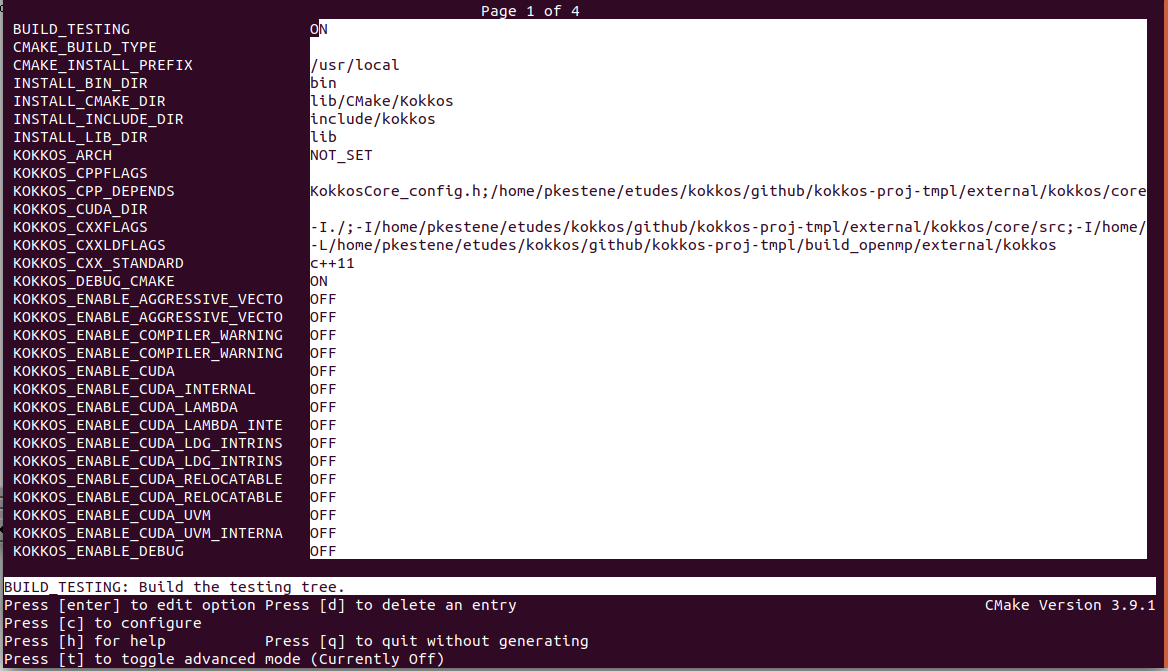
\includegraphics[width=7cm]{images/ccmake_kokkos}
    \end{center}
  \item command line interface : \texttt{cmake}
    \texttt{mkdir build\_openmp; cd build\_openmp; ccmake -DKOKKOS\_ENABLE\_OEPNMP ..}
  \item How to build ? for OpenMP / CUDA ?
  \end{itemize}

\end{frame}
  
%%%%%%%%%%%%%%%%%%%%%%%%%%%%%%%%%%%%%%%%%%%%%%%%%%%%%%%%%%%%%%%%%%%%%%%%
%%%%%%%%%%%%%%%%%%%%%%%%%%%%%%%%%%%%%%%%%%%%%%%%%%%%%%%%%%%%%%%%%%%%%%%% 
\begin{frame}[fragile=singleslide]
  \frametitle{Hands-On 3a}

  {\large \bf Activity: Use the template cmake / kokkos project}

  \begin{itemize}
  \item \textcolor{red}{\bf Clone the template project:}
  \end{itemize}
  {\small
    \begin{minted}{shell}
      git clone --recursive https://github.com/pkestene/kokkos-proj-tmpl.git
    \end{minted}
  }
  %
  \begin{itemize}
  \item \textcolor{blue}{Build the sample application (saxpy)}: use \texttt{ccmake} interface to setup the Kokkos OpenMP target; then try to setup the CUDA target (for arch Kepler37)
  \end{itemize}
  {\small
    \begin{minted}{shell}
      mkdir build_openmp; cd build_openmp; ccmake ..
      # set KOKKOS_ENABLE_OPENMP to ON
      make
    \end{minted}
  }
  % 
  \begin{itemize}
  \item \textcolor{blue}{Build the sample application (saxpy)}: repeat as above to setup the Kokkos CUDA target (for arch Kepler37)
  \end{itemize}
  %
  {\small
    \begin{minted}{shell}
      # don't forget to set environment variable CXX
      # export CXX="full path to nvcc_wrapper"
      mkdir build_cuda_kepler37; cd build_openmp; ccmake ..
      # set KOKKOS_ENABLE_CUDA to ON; set KOKKOS_ARCH
      make
    \end{minted}
  }
  %
  \begin{itemize}
  \item \textcolor{blue}{Try to add another executable}; e.g. copy of the tutorial \texttt{01\_hello\_world}
  \end{itemize}

\end{frame}



\section*{Additionnal Kokkos material}

\subsection{Use an installed version of Kokkos}
%%%%%%%%%%%%%%%%%%%%%%%%%%%%%%%%%%%%%%%%%%%%%%%%%%%%%%%%%%%%%%%%%%%%%%%% 
%%%%%%%%%%%%%%%%%%%%%%%%%%%%%%%%%%%%%%%%%%%%%%%%%%%%%%%%%%%%%%%%%%%%%%%% 
\begin{frame}[fragile=singleslide]
  \frametitle{Using an installed Kokkos (deprecated)}

  {\large \bf I strongly recommend starting using cmake to integrate kokkos in your application.} But just in case, you're still interested:
  \begin{itemize}
  \item As you will surely \textcolor{red}{\textbf{use multiple versions}} of Kokkos (OpenMP, Cuda, ...), with/without Lambda, UVM, different compilers, etc ... it will be very usefull to use some \textbf{modulefiles}.
  \item A \textcolor{blue}{\textbf{module environment}} is not a tool specific to a super-computer, it can be used on a \textbf{Desktop/Laptop} to configure an execution environment.\\
    e.g. \textcolor{blue}{\texttt{sudo apt-get install environment-modules}} (Debian/Ubuntu)
  \item \textcolor{blue}{What is a modulefiles ?}
    A simple way to set env variables to ease the use of a given software package.
  \item You will find some examples modulefiles for Kokkos in \texttt{/pwrwork/workshops/patc-201701/kokkos/modulefiles/kokkos} you can easily adapt to your own platform.
  \end{itemize}

\end{frame}

%%%%%%%%%%%%%%%%%%%%%%%%%%%%%%%%%%%%%%%%%%%%%%%%%%%%%%%%%%%%%%%%%%%%%%%% 
%%%%%%%%%%%%%%%%%%%%%%%%%%%%%%%%%%%%%%%%%%%%%%%%%%%%%%%%%%%%%%%%%%%%%%%% 
\begin{frame}[fragile=singleslide]
  \frametitle{Using an installed Kokkos (2)}

  \begin{itemize}
  \item A simple modulefiles for Kokkos should at minimum set variable \textcolor{blue}{\texttt{KOKKOS\_PATH}} pointing to the installed directory (the one which contains \textcolor{blue}{\texttt{Makefile.kokkos}}
  \item {\bf How to use Kokkos modulefiles on \textcolor{blue}{your own machine} ?} Just use the following: 
    {\small
      \begin{minted}{bash}
        # Assuming you placed the module file in
        # /somewhere_on_your_machince/modulefiles
        module use /somewhere_on_your_machince/modulefiles
        
        # e.g. load Kokkos for GPU
        module load kokkos/cuda80_gnu485_dev_k80
      \end{minted}
    }
  \item {\bf How to use Kokkos modulefiles on \textcolor{red}{ouessant} ?} Just use the following:
    {\small
      \begin{minted}{bash}
        # Assuming you placed the module file in
        # /somewhere_on_your_machince/modulefiles
        module use /pwrwork/workshops/patc-201701/kokkos/modulefiles
        # e.g. load Kokkos for GPU
        module load kokkos/cuda80_gnu485_dev_k80
      \end{minted}
    }
  \end{itemize}

\end{frame}


\subsection{Use Kokkos from Trilinos}
%%%%%%%%%%%%%%%%%%%%%%%%%%%%%%%%%%%%%%%%%%%%%%%%%%%%%%%%%%%%%%%%%%%%%%%% 
%%%%%%%%%%%%%%%%%%%%%%%%%%%%%%%%%%%%%%%%%%%%%%%%%%%%%%%%%%%%%%%%%%%%%%%% 
\begin{frame}
  \frametitle{About Kokkos in Trilinos}

  \begin{itemize}
  \item \myhref{https://github.com/kokkos/kokkos}{kokkos} is originally a subpackage of \myhref{https://trilinos.org/}{trilinos} (application framework for solving problems requiring parallel large distributed linear algebra solvers).
  \item Kokkos is the performance portable layer, to allow running Trilinos as efficiently as possible on multiple architectures.
  \item Kokkos can be build independently from Trilinos and used in other applications
  \end{itemize}

  \begin{center}
    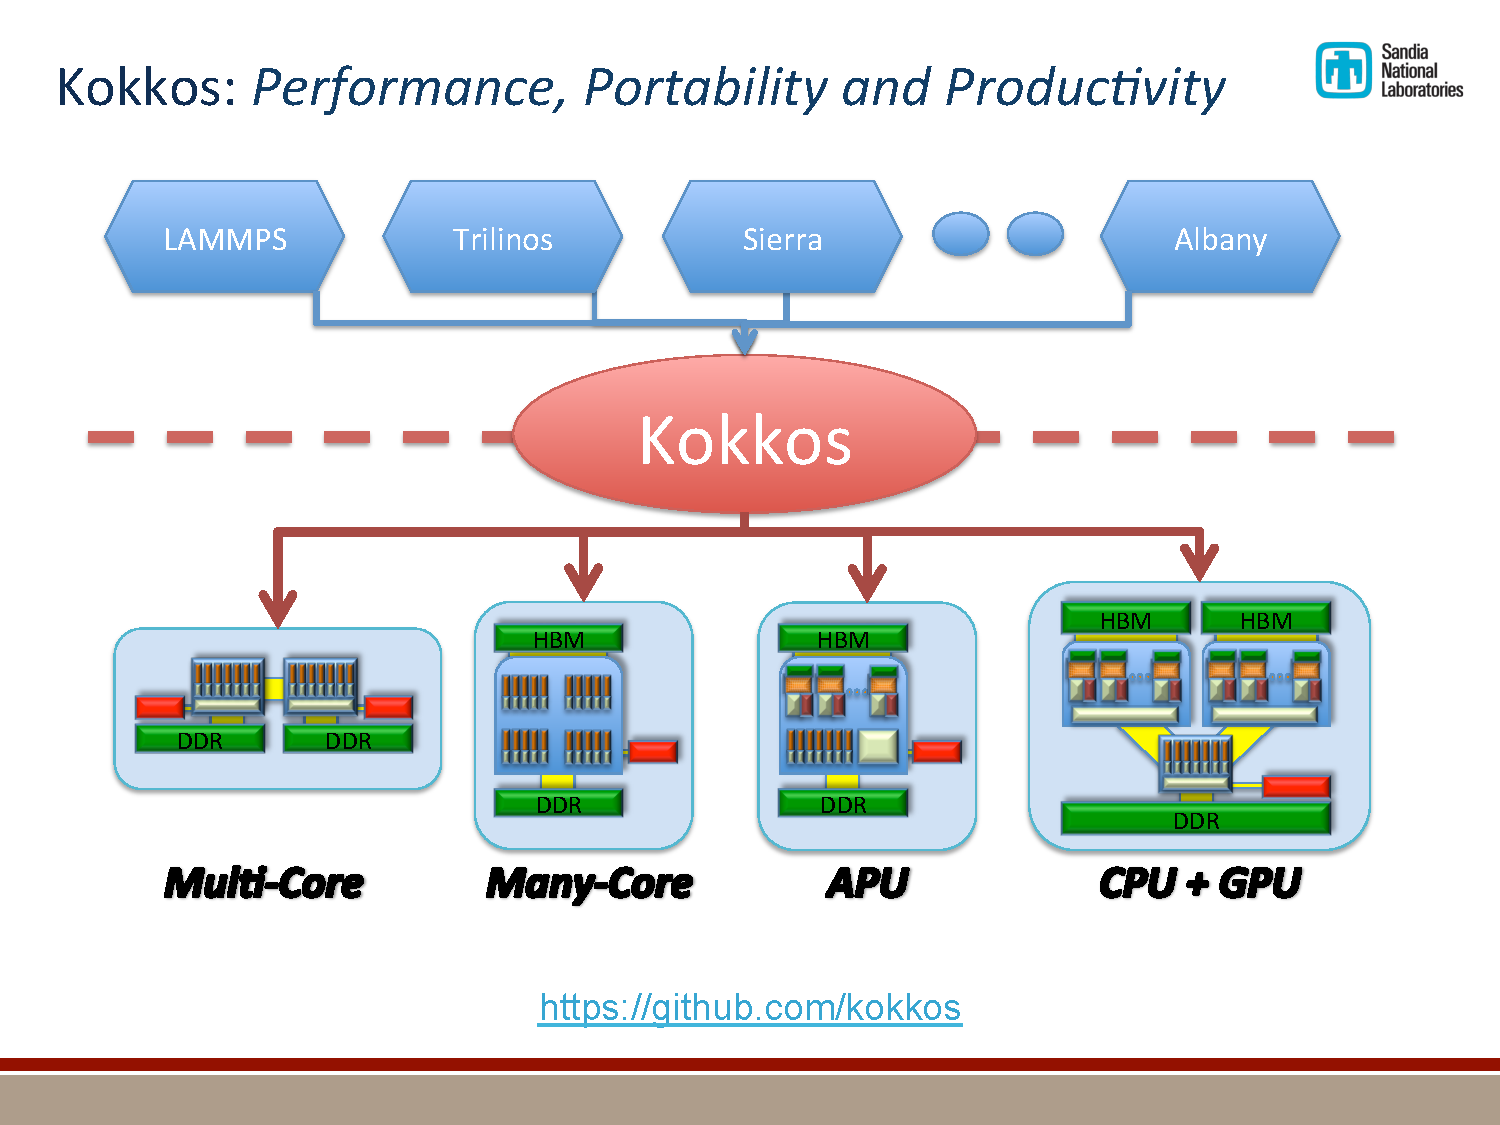
\includegraphics[width=6cm]{images/Kokkos-Multi-CoE_slide2}
  \end{center}
  
\end{frame}

%%%%%%%%%%%%%%%%%%%%%%%%%%%%%%%%%%%%%%%%%%%%%%%%%%%%%%%%%%%%%%%%%%%%%%%% 
%%%%%%%%%%%%%%%%%%%%%%%%%%%%%%%%%%%%%%%%%%%%%%%%%%%%%%%%%%%%%%%%%%%%%%%% 
\begin{frame}
  \frametitle{About Kokkos in Trilinos}

  \begin{itemize}
  \item \textbf{Build a minimal featured Trilinos with Kokkos for GPU activated} : \textcolor{red}{Tpetra + kokkos + Cuda}
    \begin{enumerate}
    \item \textbf{Example config plateform:} Ubuntu 16.04 + openmpi + cuda 8.0\\
      compiler is gcc 5.4.0
    \item \textbf{Get Trilinos sources:}\\
      \texttt{git clone https://github.com/trilinos/Trilinos.git;} \texttt{cd Trilinos; git checkout develop}
    \item \textbf{CMake configuration script:} Use the provided configuration file \texttt{configure\_tpetra\_kokkos\_cuda\_nvcc\_wrapper.sh} located in the provided archive (\texttt{doc/trilinos})\\
      this script needs slights changes (var \texttt{OMPI\_CXX} and install prefix)\\
      this script must be run in a build directory (not directly in trilinos sources).\\
      this config will build kokkos with unit tests and examples.
    \item \textbf{Build:} \texttt{make -j; make install}
    \item \textbf{Build a sample project.}
    \end{enumerate}
  \end{itemize}

\end{frame}

%%%%%%%%%%%%%%%%%%%%%%%%%%%%%%%%%%%%%%%%%%%%%%%%%%%%%%%%%%%%%%%%%%%%%%%% 
%%%%%%%%%%%%%%%%%%%%%%%%%%%%%%%%%%%%%%%%%%%%%%%%%%%%%%%%%%%%%%%%%%%%%%%% 
\begin{frame}
  \frametitle{Trilinos/Tpetra example project}

  \begin{itemize}
  \item Directory \texttt{doc/trilinos/tpetra\_example} contains a minimal example application for trilinos/tpetra. You just need to set env variable \texttt{TRILINOS\_PATH} to install directory.
  \end{itemize}
  
\end{frame}


\subsection{Custom monitoring / intrumenting / profiling}
%%%%%%%%%%%%%%%%%%%%%%%%%%%%%%%%%%%%%%%%%%%%%%%%%%%%%%%%%%%%%%%%%%%%%%%% 
%%%%%%%%%%%%%%%%%%%%%%%%%%%%%%%%%%%%%%%%%%%%%%%%%%%%%%%%%%%%%%%%%%%%%%%% 
\begin{frame}[fragile=singleslide]
  \frametitle{Kokkos profiling interface (1)}

  \begin{itemize}
  \item Kokkos provides by default a \textcolor{violet}{profiling interface} through a {\bf plugin mechanism}
  \item {\bf Usage: \textcolor{darkgreen}{profiling / monitoring / instrumenting}}
  \item From an application point of view, there is nothing to do, just provide a plugin (shared library), e.g.
    \begin{minted}{bash}
      # define path to the plugin
      export KOKKOS_PROFILE_LIBRARY=/somewhere/kp_kernel_logger.so
      # run as usal Kokkos application
    \end{minted}
  \item Examples of Kokkos profile plugins can be found at\\
    \myurl{https://github.com/kokkos/kokkos-tools}
  \end{itemize}

\end{frame}

%%%%%%%%%%%%%%%%%%%%%%%%%%%%%%%%%%%%%%%%%%%%%%%%%%%%%%%%%%%%%%%%%%%%%%%% 
%%%%%%%%%%%%%%%%%%%%%%%%%%%%%%%%%%%%%%%%%%%%%%%%%%%%%%%%%%%%%%%%%%%%%%%% 
\begin{frame}[fragile=singleslide]
  \frametitle{Kokkos profiling interface (2)}

  \begin{itemize}
  \item A Kokkos profile plugin must provide implementation for callback routines
    \begin{itemize}
    \item \texttt{kokkosp\_init\_library}
    \item \texttt{kokkosp\_finalize\_library}
    \end{itemize}
  \item A Kokkos profile interface can provide implementation for callback routines specific to a type a parallel construct, e.g. \texttt{Kokkos::parallel\_for}
    \begin{itemize}
    \item \texttt{kokkosp\_begin\_parallel\_for}
    \item \texttt{kokkosp\_end\_parallel\_for}
    \end{itemize}
    which are called every time application enters / exits this construct.
    \item see file \texttt{core/src/impl/Kokkos\_Profiling\_Interface.cpp} for a detailed list of possible callbacks.
  \end{itemize}
  
\end{frame}

% additionnal stuff
%%%%%%%%%%%%%%%%%%%%%%%%%%%%%%%%%%%%%%%%%%%%%%%%
%%%%%%%%%%%%%%%%%%%%%%%%%%%%%%%%%%%%%%%%%%%%%%%%
\begin{frame}
  \frametitle{Evaluating Peak Memory bandwidth}

  \textcolor{violet}{\Large How to determine the {\bf peak} hardware memory bandwidth of your compute platform ?}

  \begin{itemize}
  \item \textcolor{red}{\bf Multicore CPU} (e.g. Intel Skylake):
    \begin{itemize}
    \item Memory type ? e.g. DDR4-2666
    \item Number of channels ? e.g. 6
    \item Max $BW =$ \# NbOfChannel $\times$ Frequency(GHz) $\times$ BusWidth/8 (Bytes) $\times$ \# NbOfSockets
    \item e.g. on \myhref{http://www-hpc.cea.fr/fr/complexe/tgcc-Irene.htm}{TGCC/IRENE}, BW = 6 $\times$ 2.6 $\times$ 64/8 $\times$ 2 = 256 GBytes per node
    \end{itemize}
  \item \textcolor{orange}{\bf Manycore CPU} (e.g. Intel KNL):
    \begin{itemize}
    \item depends on \myhref{https://colfaxresearch.com/knl-mcdram/}{HBM configuration} (CACHE, FLAT, HYBRID)
    \item e.g. KNL on TGCC/IRENE configured in CACHE mode, BW $\geqslant 400$ GBytes/s
    \end{itemize}
  \item \textcolor{blue}{\bf NVIDIA GPU} (e.g. Pascal P100):
    \begin{itemize}
    \item Use sample application {\tt deviceQuery} to retrieve hardware spec.
    \item \# Memory Clock rate:  715 Mhz
    \item \# Memory Bus Width:   4096-bit
    \item $BW =$ 732.1 Gbytes/s
    \end{itemize}
  \item \textcolor{RoyalPurple}{\bf NVIDIA GPU} (e.g. Pascal V100):
    \begin{itemize}
    \item $BW =$ 898.0 Gbytes/s
    \end{itemize}
  \end{itemize}

% ref on KNL : http://sites.utexas.edu/jdm4372/tag/memory-bandwidth/

\end{frame}

%%%%%%%%%%%%%%%%%%%%%%%%%%%%%%%%%%%%%%%%%%%%%%%%
%%%%%%%%%%%%%%%%%%%%%%%%%%%%%%%%%%%%%%%%%%%%%%%%
\begin{frame}
  \frametitle{Evaluating Peak Memory bandwidth}

  \textcolor{violet}{\Large What about {\bf achievable} memory bandwidth ?}

  \begin{itemize}
  \item Use the stream benchmark. e.g. \myurl{https://github.com/UoB-HPC/BabelStream}
    \begin{itemize}
    \item Copy : $C[i] = A[i]$
    \item Trias : $A[i] = B[i] + scalar * C[i]$
    \end{itemize}
  \item On \textcolor{red}{\bf TGCC/Irene/Skylake} (2 sockets per node), one can measure:
    \begin{itemize}
    \item copy: $190$ GBytes/s (74 \% of peak)
    \item triad: $160$ GBytes/s (63 \% of peak)
    \end{itemize}
  \item On \textcolor{orange}{\bf TGCC/Irene/KNL} (1 socket), one can measure:
    \begin{itemize}
    \item copy: $260$ GBytes/s (65 \% of peak)
    \item triad: $330$ GBytes/s (80 \% of peak)
    \end{itemize}
  \item On \textcolor{blue}{\bf NVIDIA P100}:
    \begin{itemize}
    \item copy: $530$ GBytes/s (72 \% of peak)
    \item triad: $550$ GBytes/s (75\% of peak)
    \end{itemize}
  \item On \textcolor{RoyalPurple}{\bf NVIDIA V100}:
    \begin{itemize}
    \item copy: $650$ GBytes/s (72 \% of peak)
    \item triad: $860$ GBytes/s (95\% of peak)
    \end{itemize}
  \end{itemize}

\end{frame}


%%%%%%%%%%%%%%%%%%%%%%%%%%%%%%%%%%%%%%%%%%%%%%%%%%%%%%%%%%%%%%%%%%%%%%%% 
%%%%%%%%%%%%%%%%%%%%%%%%%%%%%%%%%%%%%%%%%%%%%%%%%%%%%%%%%%%%%%%%%%%%%%%% 
\begin{frame}
  \frametitle{Kokkos for Cuda users}

  \begin{itemize}
  \item From a pure software engineering point of view, how does Kokkos manage to turn a pur C++ functor into a CUDA kernel ?
    %
    % explain from core/src/Kokkos_Parallel.hpp
    % explain from core/src/Cuda/Kokkos_Cuda_Parallel.hpp
  \item entry point of parallel computation is through a function call to \texttt{parallel\_for} (templated by execution policy, functor, ...)
  \item \texttt{closure} : an instance of class \texttt{Kokkos::Impl::ParallelFor} is created
    % Kokkos_Parallel.hpp : line 221
    %  Impl::ParallelFor< FunctorType , policy > closure( functor , policy(0,work_count) );
  \item \texttt{Class ParallelFor} is defined in \texttt{Cuda/Kokkos\_Cuda\_Parallel.hpp}, line 456
  \item \texttt{closure.execute()} is called, which itself calls \texttt{CudaParallellaunch}
  \item Copy functor to GPU memory (constant, local or global) using Cuda API (e.g \texttt{cudaMemcpyToSymbolAsync} to copy constant memory space)
  \item finally the actual generated cuda kernel, using of the static function define (e.g. \texttt{cuda\_parallel\_launch\_constant\_memory})
    % see Kokkos_Cuda_KernelLaunch.hpp
  \end{itemize}

\end{frame}


\end{document}
